%%% pour la compilation en local 
%%% !TeX program = XeLaTeX
%%% !TeX options = -shell-escape

\documentclass[11pt,a4paper]{article}

% --- GESTION DE LA LANGUE ET DES POLICES (XELATEX) ---
\usepackage{fontspec}           % Indispensable pour XeLaTeX pour charger les polices système
\usepackage[french]{babel}      % Support de la langue française

% --- Définition des polices (à adapter) ---
\setmonofont{DejaVu Sans Mono}  % Police pour le code,
% --- GESTION DE LA GÉOMÉTRIE ET MISE EN PAGE ---
\usepackage{geometry}
\geometry{a4paper, margin=2cm} % Une seule déclaration suffit, la dernière est prise en compte

% --- PAQUETS POUR LES MATHS ---
\usepackage{amsmath}
\usepackage{amsfonts}
\usepackage{amssymb}

% --- PAQUETS GRAPHIQUES ET COULEURS ---
\usepackage{graphicx}           % Inclusion d'images
\usepackage{xcolor}             % Gestion des couleurs
\usepackage{tikz}               % Pour les schémas
\usetikzlibrary{shapes.geometric, arrows, positioning, automata, arrows.meta}
\usepackage{adjustbox}          % Pour ajuster des boîtes (comme vos figures)


% --- MISE EN FORME DU TEXTE ET TABLEAUX ---
\usepackage{enumitem}           % Pour personnaliser les listes
\setlist[itemize,1]{label=\textbullet}
\setlist[itemize,2]{label=-}
\usepackage{ulem}               % Pour barrer du texte (\sout)
\usepackage{longtable}
\usepackage{tabularx,array,booktabs}
\usepackage{float}
\usepackage{pifont}             % pour styliser les bullets
\usepackage{caption}

% --- MISE EN FORME DU CODE (MINTED) ---
% Nécessite Python + Pygments installés et la compilation avec l'option -shell-escape
\usepackage{minted} 
% L'option [outputdir=build] pour la compilation en local

\usepackage{csquotes}           % Gestion avancée des guillemets (A CHARGER APRES MINTED)

% --- LIENS HYPERTEXTE ET COULEURS PERSONNALISÉES ---
\usepackage{hyperref}
\definecolor{darkgreen}{rgb}{0.0, 0.5, 0.0}
\definecolor{darkblue}{rgb}{0.0, 0.0, 0.5}
\definecolor{darkred}{rgb}{0.5, 0.0, 0.0}
\hypersetup{
    colorlinks=true,
    linkcolor=blue,
    filecolor=magenta,      
    urlcolor=cyan,
    citecolor=blue
}

% --- COMMANDES PERSONNALISÉES ---
\definecolor{lightgray}{rgb}{0.92, 0.92, 0.92}
\newcommand{\code}[1]{\colorbox{lightgray}{\texttt{\small #1}}}
\newcommand{\var}[1]{\textit{#1}}
\newcommand{\vartype}[1]{\textcolor{darkgreen}{#1}}
\newcommand{\methodname}[1]{\textbf{\textcolor{darkblue}{#1}}}
\newcommand{\param}[1]{\code{#1}}
\newcommand{\rettype}[1]{\textcolor{darkred}{#1}}
\newcommand{\jsfunc}[1]{\textcolor{purple}{\textit{#1}}} 

\let\labelitemi\labelitemii

% --- INFORMATIONS DU DOCUMENT ---
\title{\textbf{Conception et implémentation d'un exerciseur automatique pour l'enseignement de la programmation}}
\author{ }
\date{}

\begin{document}
\maketitle

\begin{abstract}
Ce rapport présentera un outil-auteur et sa réalisation, faite dans le cadre du programme de formation GymInf. L'outil existe et propose principalement quatre fonctionnalités :
\begin{itemize}
    \item[\ding{51}] un générateur automatique (infini) de code Python valide et de niveau pédagogique adapté aux besoins définis par l'utilisateur, exécuté dans le navigateur \textit{full front-end}.
    \item[\ding{51}] un traducteur de code Python en flowchart, exécuté et affiché dans le navigateur \textit{full front-end}, et modifiable par l'utilisateur.
    \item[\ding{51}] le questionnement des élèves sur les valeurs des variables à l'issue du code proposé, avec la rétroaction réussite/échec correspondante, ainsi qu'une simulation de console d'exécution, dans le navigateur \textit{full front-end}.
    \item[\ding{51}] la constitution sur serveur d'une base de données enregistrant les codes Python générés et les interactions élèves correspondantes, laissant la possibilité de suivre individuellement l'évolution des élèves dans leurs interactions avec les codes proposés.

\end{itemize}   
Nous présenterons d'abord les contextes (professionnel, personnel, pédagogique et pratique) qui ont présidé à la réalisation de cet outil prévu pour être utilisé en classe à très brève échéance, ainsi que son architecture logique. Nous alternerons donc entre les côtés technique et fonctionnel. Le travail de développement informatique prenant une coloration didactique, nous donnerons une description logicielle de l'ensemble, ne fournissant des détails d'implémentation que sur les contributions essentielles que sont: \begin{enumerate}
    \item le générateur Javascript de codes Python tournant dans le navigateur, aléatoires mais contrôlables et de niveau pédagogique
    \item le traducteur de code Python en graphique \textit{flowchart} rendu dans le navigateur.
\end{enumerate} 
\par En raison de contraintes de temps, le dispositif n'a pas pu être passé en classe, toutefois les ambitions assumées de notre projet se situent:
\begin{itemize}
    \item chez les élèves, en développant leurs compétences stratégiques en les exerçant à une traduction entre syntaxe textuelle Python, syntaxe graphique flowchart et la sémantique associée
    \item pour la relation enseignants - apprenants, en proposant un outil-auteur adaptable et capable de proposer des codes prédéfinis par l'enseignant doublé d'un système de suivi des interactions élèves pour permettre à l'enseignant d'apporter une rétroaction différenciée au niveau individuel
    \item chez les enseignants, en proposant un outil évolutif sur lequel collaborer et donnant les moyens de développer une expertise didactique.
\end{itemize}
Dans un monde marqué simultanément par la massification de l'apprentissage de la programmation à tous les élèves de filière secondaire académique (gymnasiale, générale) et par une disparition progressive de la pratique de l'écriture de code comme compétence humaine socialement valorisée, il semble d'autant plus urgent de proposer des "outils conviviaux" (au sens d'Ivan Illich \textit{Tools for conviviality}, 1973) susceptibles de redonner aux futurs citoyens une capacité d'agir dans notre monde numérique.
\end{abstract}

\clearpage
\tableofcontents

\clearpage
\section{Introduction}
D'où vient le projet.

\subsection{Éléments de contexte}

\subsubsection{Contexte institutionnel}
\begin{description}
    \item[Institutionnel et pédagogique:] École secondaire genevoise; enseignement de l'informatique comme “Discipline Fondamentale” C'est-à-dire un cours obligatoire pour tous les élèves de 1ère et 2ème année avec très peu d’heures hebdomadaires pour chaque élève: massification des effectifs d’élèves pour l’enseignant, difficulté voire opposition de certains élèves face à la programmation.
    \item[Professionnel et personnel:] Ce projet rentre dans le cadre de la validation de ma formation GymInf et doit se terminer durant le semestre académique courant.
    \item[Professionnel et institutionnel:]
        \begin{itemize}
        \item Constat de l'absence d’une culture de groupe de discipline, besoin de créer une “communauté de pratique”; 
        \item Très grand nombre d'élèves pour chaque enseignant. Et donc besoin de rationaliser au maximum la pratique en créant des outils automatiques, besoin d’autonomiser les élèves dans leurs apprentissages; 
        \item Indisponibilité (technique ou budgétaire) ou inadéquation des outils existants (curriculum différent, objectifs "venus d'en haut" et nécessité de se conformer à une épreuve commune)
        \end{itemize}
\end{description}

\subsubsection{Contexte didactique: des hypothèses surtout}
\begin{enumerate}
    \item Pas d'analyse prévue de l'efficacité du dispositif par manque de temps et désynchronisation par rapport à l'année scolaire.
    \item Hypothèse forte: les intérêts multiples d'un générateur d'exercices aléatoires, pour autant que  l'aléa réponde à des critères pédagogiques fixés et contrôlables par l'enseignant et/ou par l'apprenant $\rightarrow$ grande variété des questions, évite la mémorisation de la solution sans investissement personnel, évite le \textit{plagiat de solutions}; peut permettre une différenciation (par adaptation au niveau réel ou supposé de l'élève).
    \item Hypothèse : intérêt de la représentation \textbf{flowchart} comme moyen d'apprentissage de la programmation - en plus d'être un objectif d'apprentissage (cf. \textit{computational thinking})  
    \item Hypothèses fortes: suprématie de la méthodologie PRIMM, qui peut aussi s'appliquer au langage flowchart (i.e. il existe un intérêt à faire lire et modifier des flowcharts aux élèves avant de leur faire écrire des flowcharts, c.f. toute la littérature depuis le  \textit{constructionnisme} de Papert).
\end{enumerate}

\subsubsection{Contexte pratico-pratique}
\begin{itemize}
    \item Pas de ressource spécifique allouée, pas de soutien institutionnel, nécessité d'une solution \textit{full front-end}.
    \item Défaut de connaissances personnelles dans le développement Web en général, et en particulier des technologies JavaScript apparues après 2015.
\end{itemize}

\subsubsection{Position de principe face à l'IA générative pour organiser le travail des élèves et proposer une rétroaction à leur travail}
Plusieurs raisons de refuser l'IA générative pour la génération aléatoire d'exercices peuvent être mises en avant: \begin{enumerate}
        \item l'impact écologique (climat et environnement: énergie, eau et terres rares, etc.), 
        \item l'inadéquation par rapport à une démarche scientifique "explicative et contrôlée", 
        \item les dérives sociales des géants du numérique (non respect des normes de traitement des humains engagés dans l'entrainement des modèles),
        \item la cannibalisation des communs numériques pour l'entrainement des LLM privés (appropriation de biens publics pour la constitution de profits privés, non respect des bonnes pratiques de crawlers web pour alimenter les modèles),
    \end{enumerate}
Une solution acceptable par principe aurait été la distillation d'un gros modèle produit dans des conditions \textit{fair-trade}, assez frugale pour tourner sur un serveur interne à l'école, mais c'est un autre sujet qui ne rentre pas dans le cadre de ce travail. Mettre dans les mains des élèves un outil basé sur l'API d'un modèle commercial, performant mais en voie de monétisation, reste inconcevable tant cela enfreindrait les principes énoncés ci-dessus tout en exposant les élèves au risque de les instrumentaliser dans le développement commercial des fournisseurs d'IA générative au prétexte de les instrumenter.

\subsection{Objectifs fonctionnels}
Ces objectifs apparaissent comme des conclusions ($\Rightarrow$) de la section précédente.

\subsubsection{Un éditeur Python...}
\begin{enumerate}
    
    \item Une fenêtre pour afficher du code Python $\Rightarrow$ besoin de recevoir du code Python de façon programmatique (voir plus loin "Générateur de codes")
    
    \item Implémentation de la méthode PRIM(M) $\Rightarrow$ besoin d'un outil dynamique permettant de donner un feedback instantané
    
    \item Encore un corollaire: besoin d'un outil permettant d'interpréter Python, qui puisse "résister" un minimum à l'apprenant afin que celui-ci s'y confronte, qui permette à l'apprenant de s'investir et d'investiguer en modifiant le code $\Rightarrow$ autres besoins ci-dessous
    
    \item Encore un corollaire: besoin d'un outil permettant de tester l'élève de façon adaptée aux objectifs controlables par l'enseignant $\Rightarrow$ autres besoins ci-dessous

    \item Un affichage "joli" pour engager tous les élèves, et pour ressembler aux \textit{IDE} que rencontreront les élèves les plus motivés, et pour ensuite pouvoir bénéficier de fonctionnalités utiles dans un cadre pédagogique, comme l'aplatissement de blocs voire l'auto-complétion.
    
\end{enumerate}
        
\subsubsection{... mais un éditeur augmenté + un rendu flowchart}
\begin{enumerate}
    
    \item Besoin d'interactions entre le DOM et l'interprétation du code Python: 
    \begin{enumerate}
        \item réception des choix utilisateurs par l'UI pour les passer à la génération de scripts; 
        \item retour des valeurs attendues et/ou des erreurs attendues vers la page; 
        \item lecture des réponses élèves pour comparaison avec les valeurs \& erreurs attendues; 
        \item affichage du feedback approprié selon étape précédente.
    \end{enumerate}
    
    \item Possibilité d'enregistrer le script sur un support (un bouton \code{Download} de sauvegarde) $+$ Possibilité de revenir au script généré (un bouton \code{Reload}) annulant les modifications apportées par l'élève depuis la génération, pour investir les dimensions "Investigate" et "Modify" du modèle PRIMM.

    \item Créer le rendu flowchart pour les codes valides:
    A priori, deux options étaient envisageables:\begin{itemize}
        \item \textbf{Soit} à la génération du script, flowchart statique (plus facile car le rendu flowchart est encapsulé avec la génération du code.
        \item \textbf{Soit} dynamique, modifiable en continu avec le code Python modifiable (besoin d'ajouter encore un bouton: alourdit l'UI qui devient moins lisible).
    \end{itemize}
    La première option aurait été en contradiction avec le point précédent, qui cherche à inciter l'investigation chez les élèves! aussi c'est la seconde option qui a été choisie.
\end{enumerate}

\subsubsection{Un générateur de codes Python, de questions pertinentes, de valeurs \& \texorpdfstring{\sout{d'erreurs attendues}}{d'erreurs attendues}}
\begin{enumerate}
    
    \item Besoin de choisir les constructions utilisées dans la génération du script qui servira de support à l'exercice \par $\Rightarrow$ besoin de fixer maintenant les types (de base) à utiliser ? Si possible une approche modulaire (très \textit{méta}) capable de s'adapter à l'ajout de fonctionnalités ultérieures (facile à dire...)

    \item Idées: en constantes une liste pré-existante de noms de variables avec leurs types parmi lesquelles choisir de façon aléatoire, et pour chaque variable un choix aléatoire de valeurs prises parmi un ensemble pré-défini qui s'ajuste selon niveau de difficulté choisi

    \item Besoin de contrôler l'aléa pour assurer une plus-value pédagogique \par $\Rightarrow$ finalement utiliser un ensemble de \textit{templates} à remplir pour chaque classe d'exercices à générer ? (plutôt qu'une approche grammaticale du langage) \par $\Rightarrow$ abandonner l'idée de générer des programmes réalistes avec définition de fonction, appels à \texttt{input} ou à \texttt{print}?
    
    \item Idées pour faire d'un script un véritable exercice: prédéfinir les questions à poser aux élèves selon le \textit{template} choisi (\textit{aka} la classe d'exercices)\par Exemples: "Quel est le nombre de passages dans la boucle?" si une boucle est choisie, "Combien de fois le bloc $xyz$ a-t-il été exécuté?" si des boucles imbriquées ont été choisies, etc. 
    
    \item Besoin de générer les valeurs attendues et des \textit{erreurs attendues} signifiantes afin de pouvoir fournir un feedback à valeur ajoutée  \par $\Rightarrow$ Idée plus radicale: se limiter à des affectations de valeurs (les questions aux élèves se limiteraient à "Valeur de x = ...", "valeur de y = ...")

    \item Préparer des questions "Comment serait modifiée la valeur si ... \textit{(ici la modification à prévoir)} ?" en plus, pour renforcer/tester la compréhension.
    
    \item Besoin de contrôler l'impossibilité de générer un script invalide pour le rendre en flowchart \textbf{VS.} la possibilité de générer un script invalide \textbf{exprès} comme variable didactique, et si oui, selon quelles erreurs permises? (Division par zéro? Index Error?) 
    
    \item A décider: la génération d'exercices "Chercher l'erreur" comme bonus, y compris erreurs syntaxiques? Un intérêt pédagogique avéré mais secondaire par rapport à mes objectifs curriculaires: le débogage
    
\end{enumerate}

\subsection{Applications similaires et sources d'inspiration}
L'objectif poursuivi a été de proposer aux enseignants d'investir en un seul outil les dimensions Predict, Run, Investigate et Modify de l'approche PRIMM d'introduction à la programmation. \par L'application présentée dans ce travail de mémoire diffère des applications existantes par son panachage unique (à ma connaissance) de plusieurs aspects :
\begin{itemize}
    \item le travail demandé aux élèves, \textbf{de lecture et traçage systématique de code, avec traduction de la syntaxe en flux sémantique}, alors que les outils connus actuellement demandent généralement d'écrire du code
    \item le caractère \textbf{automatique}, aléatoire et infini, contrôlable mais non éditorialisé
    \item la possibilité d'alterner entre \textbf{les langages Python et flowchart}, en ayant à l'écran les noms théoriques des éléments syntaxiques
    \item la possibilité avec la version serveur de tracer \textbf{le parcours des élèves} (leur investissement, leur ténacité, etc.), leurs \underline{réussites/échecs individuels avec une granularité fine} (au niveau de la valeur de chaque variable) \underline{sans bloquer les élèves face à un échec!}
\end{itemize} .

\subsubsection{Des outils auteurs}
Les outils auteurs sont des logiciels permettant à des non-développeurs (souvent des enseignants ou des concepteurs pédagogiques) de créer des contenus d'apprentissage interactifs sans écrire de code. Ils proposent généralement des modèles d'activités (quiz, glisser-déposer, etc.) à assembler.

\begin{description}
    \item[Exemple : H5P] \url{https://h5p.org/} (consulté le 5 août 2025)
    \item[Exemple : moodle] \url{https://moodle.com/} (consulté le 5 août 2025) \\
    H5P et moodle sont des frameworks open-source très populaires qui permettent de créer une grande variété de contenus interactifs directement intégrables dans des plateformes existantes. L'enseignant choisit un type d'activité (ex: "Fill in the Blanks") et remplit des champs de formulaire pour créer l'exercice.
    
    \item[Différenciation :] Notre application se distingue fondamentalement par sa \textbf{spécialisation et sa capacité de génération et de traduction en flowchart}. Alors qu'un outil auteur comme H5P demande à l'enseignant de fournir lui-même le contenu (le code Python, les questions), notre outil \textit{génère ce contenu de manière procédurale}. C'est un outil auteur \textit{spécifique au domaine} de la syntaxe Python, qui ne fournit pas des modèles d'exercices vides mais produit l'exercice (code + questions) lui-même, en fonction de contraintes pédagogiques.
\end{description}

\subsubsection{Des cours et tutoriels en ligne}
Cette catégorie regroupe les sites web qui proposent des parcours d'apprentissage structurés, souvent sous forme de textes, d'exemples et d'exercices intégrés. Leur but est de guider l'apprenant de façon réfléchie à travers un curriculum défini.

\begin{description}
    \item[Exemple : AlgoPython] \url{https://algopython.fr/} (consulté le 5 août 2025) \\
    AlgoPython est un site de référence dans le monde francophone pour l'apprentissage de Python. Il propose un cours très structuré, allant des bases de la syntaxe à des notions plus avancées, avec de nombreux exemples et des exercices à réaliser.
    
    \item[Différenciation :] La principale différence réside dans la nature du contenu et la possibilité offerte à l'élève d'expérimenter. AlgoPython propose un \textbf{contenu fixe et éditorialisé}, conçu pour être suivi de manière linéaire. Notre outil, à l'inverse, est un \textbf{générateur de contenu à la demande et non-linéaire}, offrant la possibilité supplémentaire de modifier le contenu et de l'exporter. Notre outil ne propose pas plus de cours que le seul nom des éléments syntaxique, mais est une source inépuisable d'exemples uniques sur des points de syntaxe précis, que l'enseignant peut utiliser pour illustrer une notion spécifique ou créer un exercice ponctuel.
\end{description}

\subsubsection{Des IDE pédagogiques}
Les Environnements de Développement Intégrés (IDE) pédagogiques sont des versions simplifiées des outils professionnels, conçues pour les débutants. Ils mettent l'accent sur la clarté, la visualisation de l'exécution et des messages d'erreur plus compréhensibles.

\begin{description}
    \item[Exemple : Thonny] \url{https://thonny.org/} (consulté le 5 août 2025) \\
    Thonny est un IDE Python pour débutants très apprécié. Il inclut un débogueur visuel simple qui permet de suivre l'exécution pas à pas, d'inspecter les variables et de comprendre le fonctionnement de la pile d'appels. Il doit être installé sur l'ordinateur de l'utilisateur.
    
    \item[Différenciation :] La finalité est différente. Thonny est un \textbf{environnement pour écrire et déboguer du code}. Notre application est un \textbf{générateur d'exercices pour lire et analyser du code valide}. Bien que notre outil intègre un éditeur, son but n'est pas la création de projets mais l'analyse et la modification de fragments de code (pour les phases "Run", "Investigate" et "Modify" du modèle PRIMM). De plus, notre solution de génration \& traduction est \textit{full front-end}, ne nécessitant aucune installation, contrairement à un IDE de bureau comme Thonny.
\end{description}

\subsubsection{Des plateformes pédagogiques}
Ces plateformes sont des écosystèmes complets qui intègrent un IDE en ligne, la gestion de cours, des devoirs, et souvent une infrastructure serveur pour exécuter le code et procéder à une évaluation automatique.

\begin{description}
    \item[Exemple : Replit] \url{https://replit.com/} (consulté le 5 août 2025) \\
    Replit est une plateforme en ligne extrêmement puissante qui fournit un IDE collaboratif dans le cloud pour des dizaines de langages. Elle permet aux enseignants de créer des classes, de distribuer des devoirs avec des tests unitaires pour l'auto-correction, et aux élèves de développer et d'héberger des projets complets.

    \item[Exemple : Codex (La Forge Numérique)] \url{https://codex.forge.apps.education.fr/} (consulté le 5 août 2025) \\
    Codex est une plateforme d'exercices et d'évaluation développée pour les écoles du secondaire (lycée français). Elle permet aux enseignants de créer des épreuves de programmation sécurisées, où les élèves soumettent leur code qui est ensuite évalué par des tests automatiques dans un environnement contrôlé.
    
    \item[Différenciation :] Notre application est volontairement \textbf{plus légère, plus ciblée sur l'expérimentation autonome par l'élève et axée sur la formation plutôt que l'évaluation}. Contrairement à Replit ou Codex, qui sont des solutions lourdes, forcément basées sur une infrastructure client-serveur et requérant des comptes, notre outil peut fonctionner comme une application web statique, sans serveur d'exécution grâce à Pyodide, donc anonyme, et conçue pour une tâche unique : générer des exercices ponctuels. Il n'a pas vocation à gérer un cours ou à organiser des examens, mais à fournir une ressource formative que l'enseignant peut intégrer dans son propre cheminement.
\end{description}

\subsubsection{Des défis pédagogiques}
Ces sites proposent des collections de problèmes ou "défis" de programmation que l'utilisateur doit résoudre en écrivant du code. L'accent est mis sur la résolution de problèmes et la validation algorithmique.

\begin{description}
    \item[Exemple : Codewars] \url{https://www.codewars.com/} (consulté le 5 août 2025) \\
    Codewars propose une approche ludique où les développeurs améliorent leurs compétences en résolvant des défis de programmation appelés "kata". L'utilisateur doit écrire une fonction qui passe une série de tests cachés.

    \item[Exemple : Projet Euler] \url{https://projecteuler.net/} (consulté le 5 août 2025) \\
    Le Projet Euler est une série de problèmes mathématiques complexes qui nécessitent des solutions de programmation efficaces. L'objectif est de trouver la bonne réponse numérique au problème, la qualité du code n'étant pas évaluée.

    \item[Exemple : Exercism] \url{https://exercism.org/} (consulté le 5 août 2025) \\
    Exercism se distingue en proposant des parcours d'apprentissage pour de nombreux langages. Après avoir résolu un problème, l'élève peut soumettre sa solution pour recevoir des commentaires et des conseils de la part de mentors bénévoles, mettant l'accent sur la qualité et l'\textit{idiomaticité} du code.
    
    \item[Différenciation :] La démarche pédagogique est inversée. Sur ces plateformes, le \textbf{problème est fourni} et l'élève doit \textbf{produire le code}. Dans notre application, le \textbf{code est fourni} et l'élève doit \textbf{analyser son comportement} (ex: prédire la valeur finale des variables). L'objectif n'est pas de tester la capacité à concevoir un algorithme, mais de renforcer la compréhension de la sémantique des constructions du langage. De plus, le contenu de notre outil est généré dynamiquement selon les besoins de l'enseignant, alors que les défis de ces plateformes sont des problèmes fixes (éventuellement créés par la communauté).
\end{description}

\subsubsection{Des sources d'inspiration}
A citer également :
\begin{itemize}
    \item La source d'inspiration pour l'utilisation du \textit{Control Flow Graph} de Python fourni par le module \code{ast} :  \url{https://www.fuzzingbook.org/html/GrammarFuzzer.html}
    \item Un papier universitaire présentant une initiative de génération automatique d'exercices dans le cadre de l'apprentissage de la programmation : \url{https://arxiv.org/abs/2205.11304}
    \item Un générateur de scripts Python, totalement aléatoire et intégrant un très grand nombre d'éléments syntaxiques : \url{https://github.com/radomirbosak/random-ast}
    \item Le célèbre visualiseur d'exécution de bouts de codes : \url{https://pythontutor.com/}
\end{itemize} 
\par En conclusion, la multitude des ressources pédagogiques disponibles est une source inépuisable d'inspiration, et de possible évolution, pour une prochaine version de l'outil proposant une génération sémantique (\textit{TBC}...)

\clearpage
\section{Présentation générale de l'application}
Dans cette partie : l'interface, l'architecture interne et les choix technologiques. \\

% On ouvre une minipage qui ne sera pas coupée.
\begin{minipage}{\textwidth}
\subsection{L'UI: la page \textit{Front end}}

\begin{figure}[H]
    \centering
    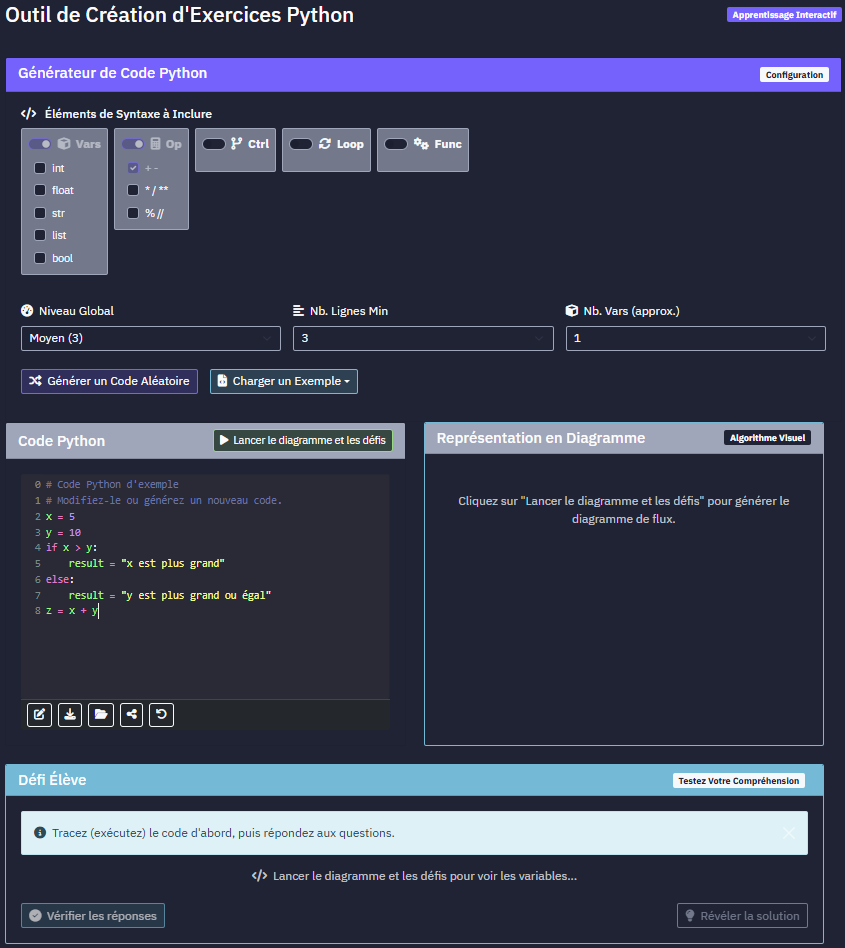
\includegraphics[width=0.99\textwidth, keepaspectratio]{app_vide.png}
    \caption{Présentation générale de l'application, vierge}
    \label{app_vide}
\end{figure}
\end{minipage}

\clearpage
\begin{minipage}{\textwidth}
\subsubsection{Les interactions entre objets : entre les \textit{cards}, entre les \textit{divs}...}

\begin{figure}[H]
    
    \centering
    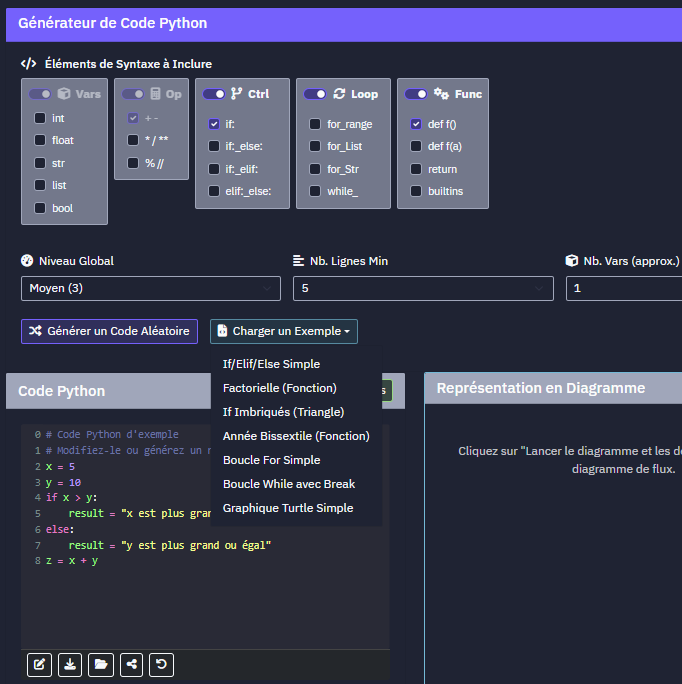
\includegraphics[width=0.8\textwidth, keepaspectratio]{app_choix.png}
    \captionof{figure}{Présentation des éléments de choix de génération ou de chargement}
    \label{app_choix}
\end{figure}

\begin{itemize}
    \item Les \textit{checkboxes} de choix des éléments syntaxiques s'affichent lorsque la \textit{card} est sélectionnée (si 'Ctrl' est sélectionnée, il y a forcément un 'if' et si 'Func' est sélectionnée, le code généré montrera au moins une 'def' de fonction).
    \item Certains choix de \textit{checkboxes} en impliquent d'autres (exemple: si 'elif:\_else' est sélectionné, le générateur de code fonctionnera forcément comme si un 'if:\_elif' avait aussi été sélectionné) $\Rightarrow$ l'interface rend visible cette logique
    \item Certains choix de structures rendent plus naturels certains choix de types de variables: l'interface rend l'utilisateur attentif par ajout d'une classe bootstrap sur l'élément concerné
\end{itemize}

\end{minipage}

\begin{figure}
    \centering
    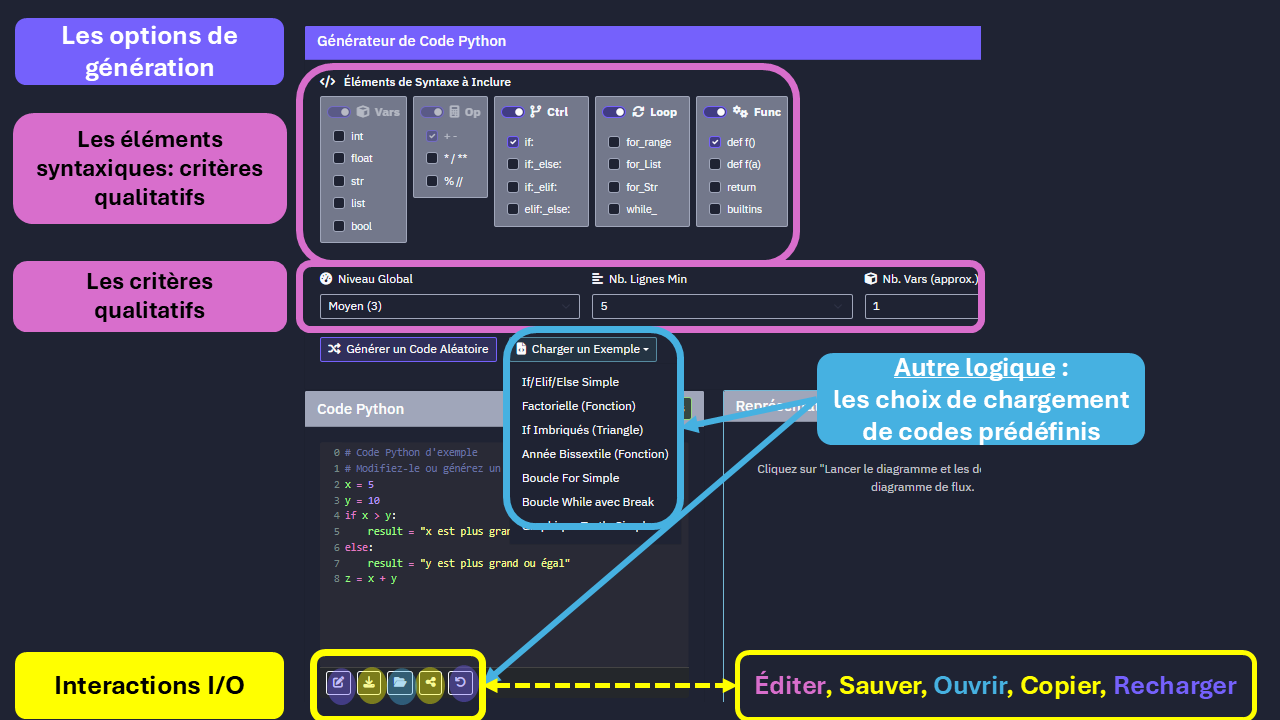
\includegraphics[width=\textwidth, keepaspectratio]{app_choix_def.png}
    \caption{Présentation des éléments de choix}
    \label{app_choix_def}
\end{figure}

\subsection{L'architecture globale (en coulisse)}

\subsubsection{Résumé en 4 phrases}
Le fonctionnement du générateur repose sur une interaction entre l'interface utilisateur (HTML - CSS - JavaScript) permettant de définir les options et le moteur de génération de code (JavaScript) qui écrit sur la page dans l'éditeur de script CodeMirror. 
\par Le fonctionnement du visualiseur flowchart se base lui sur cette chaîne de code générée, pour la traduire en un AST (Python fourni par l'environnement Pyodide) pour en extraire une sémantique traduite en une syntaxe Mermaid passée au navigateur pour être rendue sous forme graphique par Mermaid.js  
\par La partie "Défi" (avec l'interrogation des élèves sur la valeur des variables) est basée sur l'exécution du code (chaîne Python) dans le navigateur par Pyodide pour connaitre les variables à évaluer puis alimenter l'interface avec leur valeur et ainsi pouvoir proposer une rétroaction (HTML - CSS/bootstrap - JavaScript).
\par
Enfin, une partie indépendante de l'application \textit{full front-end} a été pensée pour enregistrer (\textit{journaliser}) dans une base de données relationnelle les codes générés et les interactions élèves qui ont découlé de la partie "Défi".

\subsubsection{Résumé en 1 schéma}
Le processus global peut se schématiser comme ceci: (voir page suivante selon place disponible...)

\begin{figure}[ht]
%\centering
\begin{adjustbox}{center,max width=\linewidth}
\begin{tikzpicture}[node distance=1.8cm, auto]
% Définition des styles
    \tikzstyle{block} = [rectangle, draw, fill=blue!20, text width=10em, text centered, rounded corners, minimum height=3em]
    \tikzstyle{action} = [rectangle, draw, fill=green!20, text width=8em, text centered, rounded corners, minimum height=2.5em]
    \tikzstyle{output} = [rectangle, draw, fill=orange!20, text width=8em, text centered, rounded corners, minimum height=2.5em]
    \tikzstyle{server} = [rectangle, draw, fill=yellow!20, text width=8em, text centered, rounded corners, minimum height=2.5em]
    \tikzstyle{line} = [draw, -latex']
    
    % Placement des nœuds de base: l'interface
    \node [block] (ui) {Interface utilisateur\\(layout.html)};
    \node [action, below of=ui, yshift=-0.5cm] (config) {Configuration des options};
    \node [block, below of=config, yshift=-0.5cm] (mainjs) {main.js};
    
    % Branches pour générer et lancer
    \node [action, below left of=mainjs, xshift=-4cm, yshift=-1cm] (generate) {Bouton "Générer un Code Aléatoire"};
    \node [action, below right of=mainjs, xshift=4cm, yshift=-1cm] (run) {Bouton "Lancer le diagramme et les défis"};
    
    % Nœuds liés à la génération de code
    \node [block, below of=generate, yshift=-0.5cm] (codegen) {code-generator.js};
    \node [output, below of=codegen, yshift=-0.5cm] (code) {code généré};
    \node [server, below of=code, yshift=-0.5cm] (logcode) {Code journalisé};
    
    % Nœuds liés au flowchart
    \node [block, below of=run, xshift=-2cm, yshift=-0.5cm] (flowgen) {flowchart-generator.js};
    \node [block, below of=flowgen, yshift=-0.5cm] (mycfg) {MyCFG.py via Pyodide};
    \node [output, below of=mycfg, yshift=-0.5cm] (flowchart) {Diagramme de flux};
    
    % Nœuds liés au défi
    \node [block, below of=run, xshift=2cm, yshift=-0.5cm] (runtrace) {runAndTraceCode\\ForChallenge()};
    \node [output, below of=runtrace, yshift=-0.5cm] (challenge) {Défi élève};
    \node [server, below of=challenge, yshift=-0.5cm] (loganswers) {Interaction élève journalisée};
    
    % Connexions
    \path [line] (ui) -- (config);
    \path [line] (config) -- (mainjs);
    \path [line] (mainjs) -- (generate);
    \path [line] (mainjs) -- (run);
    \path [line] (generate) -- node[left] {appelle} (codegen);
    \path [line] (codegen) -- node[left] {generateRandomPythonCode()} (code);
    \path [line] (run) -- (flowgen);
    \path [line] (run) -- (runtrace);
    \path [line] (flowgen) -- node[left] {triggerFlowchartUpdate()} (mycfg);
    \path [line] (mycfg) -- node[left] {to\_mermaid()} (flowchart);
    \path [line] (runtrace) -- (challenge);
    \path [line] (code) -- (logcode);
    \path [line] (challenge) -- (loganswers);
    
    % Connexions courbes ABANDONNÉES
%    \path [line] (code)      edge[bend left=30]  node[above] {affiché dans l'éditeur}   (ui);
 %   \path [line] (flowchart) edge[bend right=45] node[below] {affiché dans le panneau}  (ui);
  %  \path [line] (challenge) edge[bend right=60] node[below] {affiché dans le panneau}  (ui);
\end{tikzpicture}
\end{adjustbox}
\caption{Architecture détaillée de l'exerciseur automatique}
\label{fig:architecture}
\end{figure}

\subsection{Les technologies et techniques utilisées}
\subsubsection{Le navigateur: CodeMirror, Mermaid-js, Bootstrap et Font-Awesome}
\subsubsection{Pyodide: environnement Python pour le navigateur}
\subsubsection{L'extension \textit{serveur}: requêtes AJAX (JS) traitées par Flask (Python)}
\begin{enumerate}
    \item Les événements enregistrés en BDD (journalisés)
    \item La sécurité : confidentialité et anonymat
\end{enumerate}
Les événements enregistrés en BDD (journalisés): generation d'un code.
Amélioration UX : méthode P-R-G: POST-REDIRECT-GET pratique standard pour éviter le problème de soumission multiple des formulaires et ce qui rend donc l'application plus robuste face aux comportements des utilisateurs comme le rafraîchissement de page ou l'utilisation du bouton "retour" du navigateur.

\clearpage
\section{Présentation de la génération automatique du code}
C'est la branche gauche dans la figure \ref{fig:architecture}.

\subsection{Résumé de la logique}

\subsubsection{Organisation des fonctions}

Pour améliorer la clarté, proposons la structuration suivante:
Voir Figure~\ref{fig:proposed_architecture}.

\begin{figure}[htbp]
\centering
\begin{tikzpicture}[node distance=1.5cm, auto]
    % Définition des styles avec la syntaxe moderne \tikzset
    \tikzset{
        block/.style = {rectangle, draw, fill=blue!20, text width=10em, text centered, rounded corners, minimum height=3em},
        phase/.style = {rectangle, draw, fill=green!20, text width=8em, text centered, rounded corners, minimum height=2em},
        line/.style  = {draw, -latex'}
    }
   
    % Phases principales - avec beaucoup plus d'espace entre elles
    \node [phase] (phase1) {1. Initialisation};
    \node [phase, below of=phase1, yshift=-1cm] (phase2) {2. Planification};
    \node [phase, below of=phase2, yshift=-3cm] (phase3) {3. Génération};
    \node [phase, below of=phase3, yshift=-3cm] (phase4) {4. Finalisation};
    
    % Fonctions de l'étape 1
    \node [block, right of=phase1, xshift=5cm] (init) {Initialisation des variables et constantes};
    
    % Fonctions de l'étape 2 - Alignées verticalement avec leur phase
    \node [block, right of=phase2, xshift=5cm] (plan1) {calculateRequiredLines};
    \node [block, below of=plan1, yshift=-1cm] (plan2) {planVariables};
    
    % Fonctions de l'étape 3 - Alignées verticalement avec leur phase
    \node [block, right of=phase3, xshift=5cm] (gen1) {ensureVariables};
    \node [block, below of=gen1, yshift=-1cm] (gen2) {generateStructures};
    
    % Fonctions de l'étape 4 - Alignées verticalement avec leur phase
    \node [block, right of=phase4, xshift=5cm] (final1) {addFiller};
    \node [block, below of=final1, yshift=-1cm] (final2) {verifyVariables};
    
    % Connexions
    \path [line] (phase1) -- (phase2);
    \path [line] (phase2) -- (phase3);
    \path [line] (phase3) -- (phase4);
    \path [line] (phase1) -- (init);
    \path [line] (phase2) -- (plan1);
    \path [line] (phase2) -- (plan2);
    \path [line] (phase3) -- (gen1);
    \path [line] (phase3) -- (gen2);
    \path [line] (phase4) -- (final1);
    \path [line] (phase4) -- (final2);
\end{tikzpicture}
\caption{Architecture proposée pour le générateur}
\label{fig:proposed_architecture}
\end{figure}


\subsection{Cycle de vie des variables}

\begin{enumerate}
    \item \textbf{Planification}: Les variables sont planifiées selon les besoins (options utilisateur et structures)
    \item \textbf{Déclaration}: Les variables sont déclarées dans le code avec une valeur initiale
    \item \textbf{Utilisation}: Les variables sont utilisées dans les structures de contrôle
    \item \textbf{Vérification}: Toutes les variables utilisées sont bien déclarées
\end{enumerate}

L'argument \code{options} sera la structure regroupant les choix faits par l'utilisateur dans l'interface, sous la forme d'un ensemble de clé: valeur, chacune passée depuis html au code JS.
La fonction principale \code{generateRandomPythonCode(options)} est appelée par le \code{main.js} avec la constante \code{generationOptions} passée en paramètre.

\clearpage
\subsection{Schéma des appels de fonctions internes à l'exécution de la génération de code aléatoire}

%\textit{}:
% → : Alt + 26
% │ : Alt + 179
% └ : Alt + 192
% ├ : Alt + 195
% ─ : Alt + 196
%

\begin{verbatim}
├── code-generator.js
│   │
│   └── generateRandomPythonCode(options)
│       │
│       ├── 1. FONCTIONS UTILITAIRES & DE SUPPORT (*)
│       │   ├── safeIndent                                #1221
│       │   ├── shuffleArray                              #844
│       │   ├── getRandomInt, getRandomItem               #73, #81
│       │   ├── getValueRange                             #68
│       │   ├── generateValueForType, generateValueOfType #306, #347
│       │   ├── generateUniqueVarName, generateUniqueIteratorName #141, #89
│       │   ├── chooseAppropriateParameterNames           #1203
│       │   ├── getDefaultValueForType                    #1423
│       │   └── declareVariable                           #168
│       │
│       ├── 2. LOGIQUE DE GÉNÉRATION CENTRALE (appelée par autres fonctions)
│       │   ├── generateVariedOperation                   #1743 (logique anti-répétition incluse)
│       │   └── generateAppropriateStatement              #1225
│       │       └── generateVariedOperation*
│       │
│       ├── 3. PHASES D'EXÉCUTION (dans l'ordre d'appel)
│       │   │
│       │   ├── A. Phase de Préparation
│       │   │   ├── calculateRequiredLines                #1247
│       │   │   ├── generateInitialVariables              #366
│       │   │   ├── ensureVariablesForOptions             #1598
│       │   │   │   ├── ensureVariablesOfType             #1453
│       │   │   │   │   └── declareVariable*
│       │   │   │   └── ensureRequiredVariables           #1624
│       │   │   │       └── ensureVariableExists          #189
│       │   │   │           └── declareVariable*
│       │   │   ├── ensureListVariablesCount              #202
│       │   │   │   ├── generateDiverseList*
│       │   │   │   ├── declareVariable*
│       │   │   │   └── ensureListVariableIsUsed          #230
│       │   │   └── ensureTypeSpecificOperations          #1977
│       │   │       └── generateVariedOperation*
│       │   │
│       │   ├── B. Phase de Génération des Structures
│       │   │   └── generateControlStructures             #508
│       │   │       ├── shuffleArray*
│       │   │       ├── generateIfStatement               #848
│       │   │       │   ├── generateCondition
│       │   │       │   └── generateAppropriateStatement*
│       │   │       ├── generateForRangeLoop              #920
│       │   │       │   └── generateStructureBody
│       │   │       ├── generateForListLoop               #946
│       │   │       │   └── generateStructureBody
│       │   │       ├── generateForStrLoop                #986
│       │   │       │   └── generateStructureBody
│       │   │       ├── generateWhileLoop                 #1019
│       │   │       │   ├── generateCondition
│       │   │       │   └── generateStructureBody
│       │   │       └── generateFunction                  #1060
│       │   │           ├── chooseAppropriateParameterNames*
│       │   │           ├── generateStructureBody
│       │   │           └── ensureVariableExists*
│       │   │
│       │   ├── C. Phase de Finalisation
│       │   │   ├── ensureAllVariablesAreUsed             #1441
│       │   │   │   └── generateVariedOperation*
│       │   │   ├── addFiller (boucle de remplissage)     #1650
│       │   │   │   └── generateVariedOperation*
│       │   │   └── finalVariableCheck                    #1384
│       │   │       ├── declareVariable*
│       │   │       └── getDefaultValueForType*
│       │
│       └── ***LEGACY*** (finalVariableCheck a un rôle résiduel)
├── main.js
│   └── ... (logique de l'interface utilisateur, gestion des options)
│
└── MyCFG.py
    └── ... (logique d'analyse du code Python et de génération du diagramme)
\end{verbatim}
\newpage

\subsection{Documentation Technique du Générateur de code}
Cette section détaille le fonctionnement interne des fonctions principales du script \code{code-generator.js}. L'architecture repose sur un ensemble de fonctions orchestrées pour garantir la génération d'un code Python à la fois aléatoire, cohérent et pédagogiquement pertinent, en respectant scrupuleusement les options sélectionnées par l'utilisateur.

\begin{description}
\item[Portée:] Ces variables sont déclarées au niveau supérieur de la fonction \methodname{generateRandomPythonCode}. Grâce au mécanisme de clôture (closure) de JavaScript, elles sont accessibles et partagées par toutes les fonctions auxiliaires imbriquées, agissant comme un état centralisé et encapsulé pour une unique session de génération de code.
\item[Variables Clés:]
\begin{itemize}
\item \var{options}: \vartype{object}. Objet contenant toutes les options de configuration booléennes et numériques récupérées depuis l'interface HTML. C'est la source de vérité pour toutes les décisions de génération !
\item \var{codeLines}: \vartype{Array<string>}. Tableau servant d'accumulateur, chaque élément étant une ligne du code Python final. Le rôle des fonctions de génération est d'ajouter des lignes à ce tableau.
\item \var{declaredVarsByType}: \vartype{object}. Structure de données centrale qui catalogue les noms de toutes les variables déclarées, classées par type. Exemple: \code{{ int: ['count', 'x'], str: ['name'] }}.
\item \var{allDeclaredVarNames}: \vartype{Set<string>}. Ensemble stockant tous les noms de variables déjà utilisés. Sa nature de \textit{Set} garantit l'unicité.
\item \var{linesGenerated}: \vartype{number}. Compteur simple qui suit le nombre de lignes de code générées pour respecter la limite fixée par l'option \param{numLinesGlobal} qui définit l'objectif à atteindre \var{targetLines}: ni trop, ni trop peu.
\end{itemize}
\end{description}

\subsection*{Fonctions de Génération}

\begin{enumerate}
    \item \methodname{generateInitialVariables} \#366
    \begin{description}
        \item[Signature:] \code{() -> \rettype{void}}
        \item[Description:] Initialise le script en créant les variables explicitement demandées par l'utilisateur via les options \param{var\_...\_count}. Ajoute à la liste \var{typesToGenerate} les types et la quantité correspondante \code{"type : count"} reçus de HTML ; Parcourt \var{typesToGenerate} jusqu'à atteindre la taille demandée (le nombre de variables "count") ; Génère un nom et une valeur selon le type, par appels à \code{generateUniqueVarName} et \code{generateValueForType} ; Ajoute l'initialisation aux lignes de code Python générées ; Met à jour les catalogues centralisés des variables déclarées \var{allDeclaredVarNames} et \var{declaredVarsByType}, et le compteur linesGenerated. Une boucle de sécurité répète tant que les nombres de variables et de lignes de code n'ont pas tous les deux atteints les tailles demandées. La condition de sécurité est exactement: \code{while (allDeclaredVarNames.size $<$ Math.min(MAX\_TOTAL\_VARIABLES, options.numTotalVariablesGlobal $||$ 3) \&\& linesGenerated $<$ targetLines)}
    \end{description}

    \item \methodname{generateUniqueVarName(type)} \#141
    \begin{itemize}
        \item Renvoie un nom de variable qui n'a pas encore été utilisé, parmi l'ensemble prédéfini, pour le type passé en argument
        \item Construit un tableau des noms disponibles pour ce type, puis filtre ce tableau de noms en ne gardant que les noms qui n'ont pas encore été déclarés (c'est-à-dire qui ne sont pas présents dans le Set allDeclaredVarNames), et renvoie un nom choisi au hasard parmi ceux filtrés
        \item Si tous les noms sont pris pour ce type, en crée un nouveau par ajout de suffixe numérique
    \end{itemize} 

    \item \methodname{generateValueForType} \#306
\begin{description}
    \item[Signature:] \code{(\param{type}: \vartype{string}) -> \rettype{string | number | boolean}}
    \item[Description:] Agit comme un simple dispatcher pour obtenir une valeur littérale. Il utilise le dictionnaire \code{LITERALS\_BY\_TYPE} qui associe chaque type à une \jsfunc{fonction anonyme} génératrice de valeur.
    \textit{Note d'implémentation :} Les \jsfunc{fonctions} de ce dictionnaire capturent la variable \var{difficulty} depuis la portée parente, centralisant ainsi la gestion du niveau de complexité des valeurs générées.
\end{description} 
    
    \item \texttt{ensureVariablesForOptions} \#1598
    \begin{itemize}
        \item Pour chaque type parmi int, float, str, list, bool: si le compteur est strictement positif, alors appeler \texttt{ensureVariablesOfType} avec en paramètres le type et le compteur 
        \item Appelle \texttt{ensureRequiredVariables}
    \end{itemize}

    \item \texttt{ensureVariablesOfType} \#1453
    \begin{itemize}
        \item Idem \texttt{generateInitialVariables}, en version générique pour tout choix des arguments type et count
    \end{itemize}

    \item \texttt{ensureRequiredVariables} \#1624
    \begin{itemize}
        \item Fonction de sécurité pour gérer le cas particulier des loop\_for\_list et loop\_for\_str et cond\_if sans que les types correspondants n'aient été choisis dans l'interface
        \item Dans ces cas: appelle \texttt{ensureVariableExists} avec le type en paramètre
    \end{itemize}

    \item \texttt{ensureVariableExists(type) } \#189
    \begin{itemize}
        \item Pour le type passé en paramètre, renvoie soit un nom de variable existante (choisi au hasard parmi celles existantes de ce type dans \texttt{declaredVarsByType}) soit appelle \texttt{declareVariable} pour le type concerné
    \end{itemize}

    \item \texttt{declareVariable(type, value = null) -> name} \#168
    \begin{itemize}
        \item Pour le type passé en paramètre, renvoie un nom de variable généré par appel à \texttt{generateUniqueVarName} avec le type concerné en argument
        \item Si une valeur lui est passée en argument elle l'utilise, sinon elle déclare un objet littéral grâce au \emph{dictionnaire de fonctions} \texttt{LITERALS\_BY\_TYPE[type](difficulty, 'int')} \underline{DONC UNIQUEMENT ASSOCIÉ AU TYPE INT} mais bien dépendante de la difficulté
        \item Pour \texttt{LITERALS\_BY\_TYPE} voir \#46
    \end{itemize}
    
    \item \texttt{ensureListVariablesCount} \#202
    \begin{itemize}
        \item Boucle jusqu'à atteindre le compte attendu de listes: \underline{initialise une liste itemTypes avec ['int']} puis, si les options de variables ont été choisies par l'utilisateur, \underline{en ajoute une seule pour chacun des types requis} selon 'str', 'bool' et/ou 'float'
        \item Initialise une variable listValue par appel à \texttt{generateDiverseList(itemTypes,difficulty)} pour la passer en argument à \texttt{declareVariable} pour initialiser une variable listVar
    \end{itemize}
    
    \item \texttt{generateDiverseList(allowedTypes, difficulty) -> string} \#310
    \begin{itemize}
        \item Retourne des items séparés par des ', ' selon les allowedTypes et la difficulty passés en paramètres
        \item Selon la difficulté choisie, calule une taille et définit aléatoirement si la liste sera homogène (pour difficulté 1 à 3 ou 70\% de proba) ou non
        \item Dans le cas hétérogène, choisit le type courant à utiliser de façon non aléatoire par 
\begin{minted}{js}
typesToUse[i % typesToUse.length] 
\end{minted}
pour générer la valeur de l'item courant par appel à \texttt{generateValueOfType}
    \end{itemize}

    \item \texttt{generateValueOfType} \#347
    \begin{itemize}
        \item Cas 'int' ou 'float': retourne une valeur dans l'intervalle défini par la difficulté choisie et la fonction utilitaire \texttt{getValueRange}
        \item \underline{Cas 'str': retourne un mot aléatoire parmi ["alpha", "beta", "gamma", "delta", "epsilon", "kappa", "theta", "omega", "python", "code"]}
        \item Cas 'bool' : retourne au hasard 'True' ou 'False'
    \end{itemize}

\item \methodname{ensureListVariableIsUsed} \#230
    \begin{description}
        \item[Signature:] \code{(\param{listVarName}: \vartype{string}) -> \rettype{void}}
        \item[Description:] S'assure qu'une liste est active dans le code. Elle analyse les lignes existantes pour détecter une "utilisation significative" (une boucle sur cette liste, un accès à une de ses valeurs par indexation [i], ou un appel à une méthode \code{append} ou \code{extend}). Si aucune n'est trouvée, elle ajoute une opération simple comme un \code{.append()} pour illustrer concrètement l'usage d'une liste.
        \textit{Note d'implémentation :} Utilise un tableau de \jsfunc{fonctions anonymes} pour pouvoir générer des blocs de code potentiellement multi-lignes.  Ci-dessous un exemple réel d'utilisation, suivi d'explications sur ce tableau:
\begin{minted}{js}
const operations = [];
operations.push(() => {                 
    // Opération basique toujours disponible
    codeLines.push(`${listVarName}.append(${getRandomInt(1, 10)})`);
    linesGenerated++;
});
(...)
    // Exécuter une opération aléatoire
    getRandomItem(operations)();
\end{minted}
Le type de la variable \var{operations} est appelé tableau de fonctions anonymes en vocabulaire JS.
Ensuite l'appel \code{getRandomItem(operations)()} sélectionne et exécute une de ces "mini-recettes" de code en choisissant aléatoirement un élément parmi le tableau \var{operations}: \code{getRandomItem(operations)} sélectionne une fonction aléatoire parmi ces fonctions et les () après getRandomItem(operations) exécutent cette fonction sélectionnée. 
La fonction exécutée contient elle-même des appels à codeLines.push() qui ajoutent du code au tableau codeLines.
Cette technique permet à chaque fonction anonyme de générer un/des morceaux de code, avec des indentations et des structures conditionnelles complètes, sans se limiter à une seule ligne.
    \item[NB:] Si la condition \code{isNotDeclaration \&\& line.includes(listVarName) \&\& isSignificantUse} est vraie pour au moins une ligne, alors \code{codeLines.some()} retourne true, donc \var{isUsed} devient true, et donc le bloc conditionnel ne s'exécute pas !
    \end{description}

    \item \texttt{generateControlStructures()} \#508
    \begin{itemize}
        \item Fonction d'orchestration qui va appeler les fonctions correspondantes aux structures demandées par l'utilisateur
        \item Crée un tableau structures et y ajoute dans cet ordre les mots clés correspondants aux options choisies dans l'interface: 'if', 'for\_range', 'for\_list', 'for\_str', 'while' et 'function', puis appelle shuffleArray dessus, et parcourt le tableau mélangé pour appeler dans chacun des cas la fonction "generate{structure}" appropriée pour chacun des mots-clés
    \end{itemize}

    \item \methodname{ensureAllVariablesAreUsed} \#1441
    \begin{description}
    \item[Signature:] \code{() -> \rettype{void}}
    \item[Description:] Assure une bonne pratique de codage en évitant les variables inutilisées. Si une variable est jugée "inerte" (déclarée mais jamais lue), la fonction lui donne alors un rôle en ajoutant une opération simple si le nombre de lignes n'a pas atteint le nombre attendu, en appelant \methodname{generateVariedOperation} pour le niveau de difficulté reçu du scope global, et ajoute l'opération au script.
    \end{description}

    
    \item \methodname{generateVariedOperation} \#1743
\begin{description}
    \item[Signature:] \code{(\param{type}: \vartype{string}, \param{varName}: \vartype{string}, \param{difficulty}: \vartype{number}) -> \rettype{string}}
    \item[Description:] Moteur de génération d'opérations atomiques (une/des lignes de code). Il utilise une table de dispatch pour sélectionner une opération possible en fonction du \param{type} et de la \param{difficulty}. Il intègre une logique anti-répétition et des patchs de sécurité (ex: détection d'opérations invalides sur les chaînes) pour garantir la qualité et la variété du code.
    \item[Étape 1:] Crée d'abord une table de dispatch (un objet littéral contenant des fonctions fléchées) où chaque type passé en paramètre pointe vers un tableau de fonctions qui générent des opérations adaptées à ce type, ce qui permet de construire \code{ availableOps = operations[type]} et de choisir au hasard parmi ce tableau un opération disponbile
    \item[Étape 2:] Essaie d'ajouter une opération différente des/de la précédente plusieurs fois, si toujours sans succès: ajoute un commentaire très improbable, pris aléatoirement parmi les caractères alphanumériques (ligne \#1870)
    \item[Étape 3:] Ajoute un patch regex pour détecter les opérations arithmétiques invalides sur 'str' et les remplacer à la volée par une opération valide, sélectionnée aléatoirement parmi un tableau (ligne \#1940)
\end{description}
    
    \item \texttt{generateIfStatement} \#848
    \item \texttt{generateForRangeLoop} \#920
    \item \texttt{generateForListLoop} \#946
    \item \texttt{generateForStrLoop} \#986
    \item \texttt{generateWhileLoop} \#1019
    \item \texttt{generateFunction} \#1060

    \item \texttt{generateCondition(varTypes = ['int', 'bool', 'str', 'list'], preferExisting = true)} \#409
    \begin{itemize}
        \item Ajoute au tableau possibleConditions des conditions définies manuellement selon les types rencontrés dans varTypes passé en paramètre, puis en choisis une au hasard parmi possibleConditions.
        \item Plan B: si aucune variable existante ne peut être utilisée (exemple: le générateur de boucle while demande une condition while\_safe qui ne peut être créée avec les variables existantes), le bloc de 'fallback' va ajouter au code généré une déclaration/initialisation d'une nouvelle variable et une condition simple l'utilisant ('bool' = True|False ou 'int' > 0). Sans oublier de mettre à jour les structures declaredVarsByType, allDeclaredVarNames et le compteur linesGenerated après avoir incrémenté le compteur pour l'ajout de la variable.
    \end{itemize}


    \item \texttt{generateStructureBody(indentLevel, contextType, contextOptions = \{\})} \#551
    \begin{itemize}
        \item Fonction appelée par les générateurs de structures pour créer un corps fait d'un nombre d'instructions variable selon la difficulté, situé par indentLevel, pour une structure identifiée par contextType (qui peut être for\_range, for\_list, for\_str ou function). Différentes logiques sont implémentées pour essayer de créer un équilibre entre des opérations de base garanties, l'introduction progressive de complexité, et une variété d'opérations qui restent asez simples pour remplir le corps de la boucle.
        \item Explications sur le mapping contextOptions passé en paramètre : c'est le moyen de passer un ensemble de paramètres spécifiques au contexte (exemples: le nom de la variable de boucle loopVar, ou si un return est attendu) à la fonction generateStructureBody, sans avoir à lister une dizaine de paramètres dans sa signature!
        \item Le cas function est le context le plus complexe évidemment: la fonction se base sur le type du premier paramètre pour ajouter des opérations adaptées, écrites manuellement chacune dans l'objectif de proposer aux élèves des syntaxes variées et valides pour des opérations sur 'str', 'list', 'bool' et 'int'|'float'.
        \item Les cas des boucles 'for' utilisent une première instruction basique typique (addition d'un entier pour une variable dans un range, ajout d'un caractère pour une variable parcourant une chaine) suivie d'instructions choisies aléatoirement. Pour l'instruction basique de début de corps de boucle 'for\_range' nous avons au contraire été amenés à pallier la forte probabilité de répétition d'instructions identiques en ajoutant la génération d'un commentaire improbable, pour assurer l'unicité de chacune des lignes:
        \begin{minted}{js}
// Vérifier si cette opération est déjà présente dans le corps
if (addedOperations.has(operation)) {
    // Ajouter un commentaire unique pour la rendre différente
    const uniqueId = Math.random().toString(36).substring(2, 5);
    operation = operation.replace(/\s*#.*$/, '') + `  # var_${uniqueId}`;
                }
        \end{minted}
        \item Dans la suite du corps (de boucle ou de fonction) les instructions sont générées par appel à generateVariedOperation. Cette dernière fonction intègre déjà une logique aléatoire avec un vrai évitement des répétitions en choisissant une structure différente, plus robuste que le "patch" ci-dessus qui rend unique une instruction par simple ajout d'un commentaire. 
    \end{itemize}


    \item \methodname{finalVariableCheck} \#1384
    \begin{description}
        \item[Signature:] \code{() -> \rettype{void}}
        \item[Description:] \textit{Rôle legacy.} Cette fonction était un garde-fou dans les anciennes versions pour s'assurer que les variables "planifiées" étaient bien déclarées. Avec la nouvelle architecture où les variables sont déclarées immédiatement, son rôle est devenu mineur et elle est conservée comme une sécurité résiduelle.
    \end{description}
    
\end{enumerate}

\clearpage
\section{Présentation détaillée du traducteur automatique de code en logigramme}

\subsection{L'AST Python: théorie et PyCFG.py de \textit{Fuzzingbook}}

\subsection{Philosophie poursuivie}

\subsection{L'implémentation MyCFG.py}

La classe Python \code{ControlFlowGraph} est le composant central pour la transformation du code Python généré (une chaine) en un \textit{flowchart} (une chaine Mermaid rendue graphiquement par l'interface).

\subsection*{\methodname{\_\_init\_\_}}
\begin{description}
    \item[Signature:] \code{(\_\_init\_\_(self, code: \vartype{str})) -> \rettype{None}}
    \item[Description:] Constructeur de la classe. Initialise l'analyseur AST avec le code Python fourni et prépare les structures de données internes pour stocker les informations du graphe de flux de contrôle (ci-après \textit{flowchart}). Cette méthode est appelée une seule fois lors de la création d'une instance de \code{ControlFlowGraph}.
    \item[Variables d'instance initialisées:]
    \begin{itemize}
        \item \var{tree}: \vartype{ast.Module}. L'arbre syntaxique abstrait (AST) généré à partir du \param{code} source. C'est la structure de base que les méthodes de visite parcourront.
        
        \item \var{nodes}: \vartype{List[Tuple[str, str]]}. Liste de tuples, où chaque tuple représente un nœud du CFG sous la forme \code{(node\_id, label)}. \code{node\_id} est un identifiant unique et \code{label} est le texte affiché dans la forme (rectangulaire ou autres). Seuls les nœuds de jonctino, techniques, n'ont pas ce texte.
        
        \item \var{edges}: \vartype{Set[Tuple[str, str, str]]}. Ensemble de tuples représentant les arêtes du CFG. Chaque tuple est de la forme \code{(from\_node\_id, to\_node\_id, label)}, où \code{label} est le texte affiché sur l'arête (peut être vide). Utiliser un ensemble évite les arêtes dupliquées.
        
        \item \var{node\_counter}: \vartype{int}. Compteur entier utilisé par \code{get\_node\_id} pour générer des identifiants de nœuds uniques (par exemple, "node01", "node02"). Initialisé à 0.
        
        \item \var{loop\_stack}: \vartype{List[Tuple[str, str, str]]}. Pile utilisée pour gérer le contexte des boucles imbriquées. Chaque élément est un tuple \code{(continue\_target\_id, break\_target\_id, retest\_target\_id)} stockant les ID des nœuds cibles pour les instructions \code{continue}, \code{break}, et pour le retour au test de la condition de boucle. NB: les \code{break} ne sont pas encore bien implémentés même si l'arête est générée!
        
        \item \var{node\_labels}: \vartype{Dict[str, str]}. Dictionnaire associant un \code{node\_id} à son \code{label} textuel. Permet un accès rapide au label d'un nœud.
        
        \item \var{terminal\_nodes}: \vartype{Set[str]}. Ensemble des \code{node\_id} qui représentent la fin d'un chemin d'exécution normal (par exemple, un nœud créé pour une instruction \code{return}, \code{break}, ou \code{continue}).
        
        \item \var{node\_types}: \vartype{Dict[str, str]}. Dictionnaire associant un \code{node\_id} à son type sémantique (par exemple, "Process", "Decision", "StartEnd", "Junction"). Utilisé pour le style dans le rendu Mermaid, en évitant d'utiliser des mots-clés déjà pris.
        
        \item \var{\_function\_scope\_stack}: \vartype{List[Set[str]]}. Pile interne pour gérer les portées des fonctions (imbriquées ou non). La \textbf{"portée d'une fonction" fait ici référence à l'ensemble des nœuds du graphe de flux de contrôle (CFG) qui sont générés} lors de l'analyse du corps de cette fonction spécifique. La principale utilité est de permettre à la méthode \code{connect\_finals\_to\_end} de fonctionner correctement. Quand on est à la fin de la visite d'une fonction (dans \code{visit\_FunctionDef}), on veut s'assurer que tous les chemins d'exécution à l'intérieur de cette fonction qui n'ont pas explicitement de successeur (fins de chemin implicites ou nœuds Return) soient connectés au nœud End {NomFonction} de cette fonction spécifique, et non au End du module. Cela permet d'identifier quels nœuds appartiennent à quelle fonction pour les regrouper visuellement dans des \code{subgraph} distincts. Chaque élément de la liste est un ensemble d'ID de nœuds appartenant à une portée de fonction spécifique. Lorsqu'on commence à visiter une fonction (visit\_FunctionDef), un nouvel ensemble vide (set()) est poussé sur cette pile. \textbf{Explications}: Chaque fois qu'un nouveau nœud CFG est créé (get\_node\_id) pendant que cette fonction est en cours de visite (c'est-à-dire, pendant que son ensemble est au sommet de la pile), l'ID de ce nouveau nœud est ajouté à cet ensemble au sommet de la pile. Cela gère correctement les fonctions imbriquées : si func\_A contient func\_B, lors de la visite de func\_A, son scope est sur la pile. Quand visit\_FunctionDef est appelée pour func\_B, un nouveau scope pour func\_B est poussé par-dessus celui de func\_A. Les nœuds de func\_B vont dans le scope de func\_B. Quand la visite d'une fonction est terminée, son ensemble d'ID de nœuds est retiré (poppé) de la pile et stocké dans \code{self.all\_function\_scopes} (qui conserve tous les scopes de fonction finalisés). La dernière portée de la liste est la plus interne.
        
        \item \var{function\_subgraph\_nodes}: \vartype{Dict[str, Set[str]]}. Dictionnaire stockant, pour chaque nom de fonction, l'ensemble des ID de nœuds qui lui appartiennent. Utilisé par \code{to\_mermaid} pour créer les sous-graphes.
        
        \item \var{main\_flow\_nodes}: \vartype{Set[str]}. Ensemble des ID de nœuds appartenant au flux principal du module (hors définitions de fonctions). Utilisé par \code{to\_mermaid} pour le sous-graphe principal.
    \end{itemize}
\end{description}

\subsection*{\methodname{get\_node\_id}}
\begin{description}
    \item[Signature:] \code{(get\_node\_id(self) -> \rettype{str})}
    \item[Description:] Génère un identifiant de nœud unique basé sur \var{node\_counter}. Si l'appel se produit dans le contexte d'une fonction (c'est-à-dire si \var{\_function\_scope\_stack} n'est pas vide), l'ID du nouveau nœud est ajouté à l'ensemble des nœuds de la portée de fonction la plus interne. Sinon, il est ajouté à \var{main\_flow\_nodes}. Cette méthode est appelée par \code{add\_node} chaque fois qu'un nouveau nœud est créé.
    \item[Variables locales/modifiées:]
    \begin{itemize}
        \item \var{new\_id}: \vartype{str}. L'identifiant de nœud nouvellement généré (par exemple, "node01").
        \item Modifie \var{self.node\_counter} (incrémenté).
        \item Modifie potentiellement \var{self.\_function\_scope\_stack[-1]} ou \var{self.main\_flow\_nodes} en y ajoutant \var{new\_id}.
    \end{itemize}
\end{description}

\subsection*{\methodname{add\_node}}
\begin{description}
    \item[Signature:] \code{(add\_node(self, label: \vartype{str}, node\_type: \vartype{str} = "Process") -> \rettype{str})}
    \item[Description:] Crée un nouveau nœud avec le \param{label} et le \param{node\_type} fournis, l'ajoute aux structures de données internes du graphe (\var{self.nodes}, \var{self.node\_labels}, \var{self.node\_types}), et retourne l'ID unique du nœud créé. Appelée par les différentes méthodes de visite lorsqu'une instruction ou une structure de contrôle doit être représentée par un nœud.
    \item[Paramètres:]
    \begin{itemize}
        \item \param{label}: \vartype{str}. Le texte à afficher sur le nœud.
        \item \param{node\_type}: \vartype{str}. Le type sémantique du nœud (défaut: "Process").
    \end{itemize}
    \item[Variables locales/modifiées:]
    \begin{itemize}
        \item \var{node\_id}: \vartype{str}. L'ID du nœud créé, obtenu via \code{get\_node\_id}.
        \item Modifie \var{self.nodes}, \var{self.node\_labels}, \var{self.node\_types}.
    \end{itemize}
\end{description}

\subsection*{\methodname{add\_edge}}
\begin{description}
    \item[Signature:] \code{(add\_edge(self, from\_node: \vartype{str}, to\_node: \vartype{str}, label: \vartype{str} = "") -> \rettype{None})}
    \item[Description:] Ajoute une arête dirigée entre deux nœuds identifiés par \param{from\_node} et \param{to\_node}, avec un \param{label} optionnel. Effectue des vérifications pour éviter les arêtes invalides (nœuds non existants, auto-boucles non labellisées, arêtes sortant de nœuds terminaux non autorisés). Appelée par les méthodes de visite pour connecter les nœuds représentant le flux de contrôle.
    \item[Paramètres:]
    \begin{itemize}
        \item \param{from\_node}: \vartype{str}. L'ID du nœud de départ de l'arête.
        \item \param{to\_node}: \vartype{str}. L'ID du nœud d'arrivée de l'arête.
        \item \param{label}: \vartype{str}. Le texte à afficher sur l'arête (défaut: chaîne vide).
    \end{itemize}
    \item[Variables locales/modifiées:]
    \begin{itemize}
        \item Modifie \var{self.edges} en y ajoutant le tuple de l'arête.
    \end{itemize}
\end{description}

\subsection*{\methodname{\_is\_terminal\_ast\_node}}
\begin{description}
    \item[Signature:] \code{(\_is\_terminal\_ast\_node(self, node: \vartype{ast.AST}) -> \rettype{bool})}
    \item[Description:] Petite méthode utilitaire vérifiant si un \code{node} AST donné est un type d'instruction qui termine le flux d'exécution normal (i.e. présentement: \code{ast.Return}, \code{ast.Break}, \code{ast.Continue}). Appelée par la méthode \code{visit} pour déterminer si les nœuds CFG créés doivent être marqués comme terminaux.
    \item[Paramètres:]
    \begin{itemize}
        \item \param{node}: \vartype{ast.AST}. Le nœud AST à inspecter.
    \end{itemize}
\end{description}

\subsection*{\methodname{visit\_body}}
\begin{description}
    \item[Signature:] \code{(visit\_body(self, body: \vartype{List[ast.AST]}, entry\_node\_ids: \vartype{List[str]}) -> \rettype{List[str]})}
    \item[Description:] Traite une séquence d'instructions (un "corps" de code, comme le corps d'une fonction, d'une boucle ou d'une branche conditionnelle). Elle itère sur chaque instruction du \param{body}, la visite en utilisant les \param{entry\_node\_ids} comme points d'entrée, et gère la création de nœuds de jonction si une instruction produit plusieurs sorties non terminales et n'est pas la dernière du corps. Retourne une liste des ID de nœuds qui constituent les points de sortie finaux de ce corps. Appelée par \code{visit\_Module}, \code{visit\_FunctionDef}, \code{visit\_If}, \code{visit\_For}, \code{visit\_While}.
    \item[Paramètres:]
    \begin{itemize}
        \item \param{body}: \vartype{List[ast.AST]}. La liste des nœuds AST représentant les instructions du corps.
        \item \param{entry\_node\_ids}: \vartype{List[str]}. Liste des ID des nœuds CFG qui servent de points d'entrée pour la première instruction de ce corps.
    \end{itemize}
    \item[Variables locales/modifiées:]
    \begin{itemize}
        \item \var{active\_ids\_for\_current\_statement}: \vartype{List[str]}. Liste des ID de nœuds actifs qui servent d'entrée à l'instruction en cours de traitement ou de sortie de l'instruction précédente. Initialisée avec \param{entry\_node\_ids}, puis mise à jour après chaque instruction.
        \item \var{i}: \vartype{int}. Index de l'instruction en cours dans la boucle sur \param{body}.
        \item \var{stmt}: \vartype{ast.AST}. L'instruction AST en cours de traitement.
        \item \var{current\_stmt\_entry\_points}: \vartype{List[str]}. Sous-ensemble de \var{active\_ids\_for\_current\_statement} ne contenant que les nœuds non terminaux, servant d'entrée à l'appel de \code{visit(stmt, ...)}.
        \item \var{exits\_from\_current\_stmt\_all\_paths}: \vartype{List[str]}. Liste collectant tous les ID de nœuds de sortie retournés par \code{visit(stmt, ...)} pour tous ses points d'entrée.
        \item \var{parent\_id}: \vartype{str}. Un ID de nœud de \var{current\_stmt\_entry\_points}, passé comme parent à \code{visit(stmt, parent\_id)}.
        \item \var{exit\_nodes\_from\_stmt\_path}: \vartype{List[str]}. Les ID de nœuds de sortie retournés par un appel spécifique à \code{visit(stmt, parent\_id)}.
        \item \var{is\_last\_statement}: \vartype{bool}. Indicateur si \var{stmt} est la dernière instruction du \param{body}.
        \item \var{non\_terminal\_active\_ids}: \vartype{List[str]}. Sous-ensemble de \var{active\_ids\_for\_current\_statement} (après traitement de \var{stmt}) ne contenant que les nœuds non terminaux. Utilisé pour décider de créer une jonction.
        \item \var{junction\_id}: \vartype{str}. ID du nœud de jonction créé si nécessaire. Initialisé uniquement si plus d'un \var{non\_terminal\_active\_ids} existe et que ce n'est pas la dernière instruction.
        \item \var{pid}: \vartype{str}. Un ID de nœud de \var{non\_terminal\_active\_ids}, utilisé pour connecter ces nœuds à \var{junction\_id}.
        \item \var{terminal\_active\_ids}: \vartype{List[str]}. Sous-ensemble de \var{active\_ids\_for\_current\_statement} contenant les nœuds terminaux. Conservés lors de la création d'une jonction.
    \end{itemize}
\end{description}

\subsection*{\methodname{visit}}
\begin{description}
    \item[Signature:] \code{(visit(self, node: \vartype{ast.AST}, parent\_id: \vartype{Optional[str]}) -> \rettype{List[str]})}
    \item[Description:] Méthode de répartition principale (dispatcher) qui dirige la visite d'un \param{node} AST vers la méthode \code{visit\_<NodeType>} appropriée (par exemple, \code{visit\_If} pour un \code{ast.If}). Si aucune méthode spécifique n'existe, elle utilise \code{generic\_visit}. Après l'appel au visiteur spécifique, si le \param{node} AST est de type terminal (Return, Break, Continue), elle marque les nœuds CFG créés comme terminaux et retourne une liste vide (indiquant aucune continuation de flux normale). Sinon, elle retourne la liste des ID de nœuds de sortie produits par le visiteur. Appelée récursivement pour parcourir l'AST.
    \item[Paramètres:]
    \begin{itemize}
        \item \param{node}: \vartype{ast.AST}. Le nœud AST à visiter.
        \item \param{parent\_id}: \vartype{Optional[str]}. L'ID du nœud CFG parent auquel le(s) nouveau(x) nœud(s) créé(s) pour \param{node} doi(ven)t être connecté(s). Peut être \code{None} pour le nœud Module ou les FunctionDef de haut niveau.
    \end{itemize}
    \item[Variables locales/modifiées:]
    \begin{itemize}
        \item \var{method\_name}: \vartype{str}. Le nom de la méthode de visite spécifique (par exemple, "visit\_If").
        \item \var{visitor}: \vartype{Callable}. La référence à la méthode de visite à appeler.
        \item \var{exit\_nodes}: \vartype{List[str]}. Liste des ID de nœuds de sortie retournés par la méthode \var{visitor}.
        \item \var{node\_id} (dans la section terminal): \vartype{str}. Un ID de nœud de \var{exit\_nodes}, utilisé pour l'ajouter à \var{self.terminal\_nodes}.
        \item Modifie potentiellement \var{self.terminal\_nodes}.
    \end{itemize}
\end{description}

\subsection*{\methodname{connect\_finals\_to\_end}}
\begin{description}
    \item[Signature:] \code{(connect\_finals\_to\_end(self, target\_end\_id: \vartype{str}, scope\_node\_ids: \vartype{Optional[Set[str]]} = None) -> \rettype{None})}
    \item[Description:] Parcourt les nœuds spécifiés par \param{scope\_node\_ids} (ou tous les nœuds si \code{None}). Si un nœud dans cette portée n'a pas d'arête sortante ou s'il s'agit d'un nœud "Return", une arête est ajoutée de ce nœud vers \param{target\_end\_id}. Cela garantit que tous les chemins d'exécution (y compris les retours implicites et explicites) se terminent correctement au nœud "End" approprié (de module ou de fonction). Appelée par \code{visit\_Module} et \code{visit\_FunctionDef}.
    \item[Paramètres:]
    \begin{itemize}
        \item \param{target\_end\_id}: \vartype{str}. L'ID du nœud "End" auquel connecter les nœuds finaux.
        \item \param{scope\_node\_ids}: \vartype{Optional[Set[str]]}. Ensemble optionnel d'ID de nœuds à considérer. Si \code{None}, tous les nœuds du graphe sont vérifiés.
    \end{itemize}
    \item[Variables locales/modifiées:]
    \begin{itemize}
        \item \var{source\_nodes\_with\_outgoing\_edges}: \vartype{Set[str]}. Ensemble des ID de nœuds qui ont au moins une arête sortante.
        \item \var{nodes\_to\_check}: \vartype{Set[str]}. L'ensemble effectif des ID de nœuds à inspecter.
        \item \var{node\_id}: \vartype{str}. L'ID du nœud en cours d'inspection dans la boucle.
        \item \var{is\_return\_node}: \vartype{bool}. Vrai si le \var{node\_id} actuel est de type "Return".
        \item Modifie \var{self.edges} en ajoutant des arêtes vers \param{target\_end\_id}.
    \end{itemize}
\end{description}

\subsection*{\methodname{visit\_Module}}
\begin{description}
    \item[Signature:] \code{(visit\_Module(self, node: \vartype{ast.Module}, parent\_id: \vartype{Optional[str]} = None) -> \rettype{List[str]})}
    \item[Description:] Gère la visite du nœud racine du module (\code{ast.Module}). Crée les nœuds "Start" et "End" globaux. Sépare les définitions de fonctions des autres instructions. Visite d'abord les définitions de fonctions (qui génèrent leurs propres sous-graphes isolés), puis visite les autres instructions pour construire le flux principal du module. Enfin, connecte les points de sortie du flux principal et les fins implicites au nœud "End" global. Appelée une seule fois, au début du processus de visite, avec \param{parent\_id} à \code{None}.
    \item[Paramètres:]
    \begin{itemize}
        \item \param{node}: \vartype{ast.Module}. Le nœud AST du module.
        \item \param{parent\_id}: \vartype{Optional[str]}. Toujours \code{None} pour cette méthode.
    \end{itemize}
    \item[Variables locales/modifiées:]
    \begin{itemize}
        \item \var{start\_id}: \vartype{str}. ID du nœud "Start" du module.
        \item \var{function\_defs}: \vartype{List[ast.FunctionDef]}. Liste des nœuds AST de définition de fonction dans le module.
        \item \var{other\_statements}: \vartype{List[ast.AST]}. Liste des autres nœuds AST (non-FunctionDef) dans le module.
        \item \var{func\_def\_node} (dans la boucle): \vartype{ast.FunctionDef}. Une définition de fonction en cours de visite.
        \item \var{module\_flow\_exits}: \vartype{List[str]}. Liste des ID de nœuds de sortie du flux principal du module, retournée par \code{visit\_body(other\_statements, ...)}.
        \item \var{module\_end\_id}: \vartype{str}. ID du nœud "End" du module.
        \item \var{node\_id} (dans la boucle de connexion): \vartype{str}. Un ID de nœud de \var{module\_flow\_exits}.
    \end{itemize}
\end{description}

\subsection*{\methodname{visit\_FunctionDef}}
\begin{description}
    \item[Signature:] \code{(visit\_FunctionDef(self, node: \vartype{ast.FunctionDef}, parent\_id: \vartype{Optional[str]}) -> \rettype{None})}
    \item[Description:] Gère la visite d'un nœud de définition de fonction (\code{ast.FunctionDef}). Crée une nouvelle portée de fonction, puis les nœuds "Start NomFonction" et "End NomFonction" pour le corps de cette fonction. Visite le corps de la fonction. Collecte tous les ID de nœuds créés dans cette portée, les stocke dans \var{self.function\_subgraph\_nodes} pour le rendu en sous-graphe, puis dépile la portée. Connecte les points de sortie normaux du corps et les nœuds "Return" au nœud "End NomFonction" de cette fonction. Ne s'insère pas dans le flux du parent et retourne une liste vide. Appelée par \code{visit\_Module} ou par un autre \code{visit\_FunctionDef} (pour les fonctions imbriquées).
    \item[Paramètres:]
    \begin{itemize}
        \item \param{node}: \vartype{ast.FunctionDef}. Le nœud AST de la définition de fonction.
        \item \param{parent\_id}: \vartype{Optional[str]}. L'ID du nœud parent. \code{None} si c'est une fonction de haut niveau, ou l'ID du nœud de la fonction englobante si elle est imbriquée (Mise à jour: la version actuelle ne crée plus de nœud de déclaration dans le flux parent... seul subsiste l'appel de fonction dans le flux parent, la déclaration est représentée par un sous-graphe pour la définition de fonction).
    \end{itemize}
    \item[Variables locales/modifiées:]
    \begin{itemize}
        \item \var{func\_body\_start\_id}: \vartype{str}. ID du nœud "Start NomFonction".
        \item \var{func\_body\_end\_id}: \vartype{str}. ID du nœud "End NomFonction".
        \item \var{body\_normal\_exit\_nodes}: \vartype{List[str]}. Liste des ID de nœuds de sortie normaux du corps de la fonction.
        \item \var{node\_id} (dans la boucle de connexion): \vartype{str}. Un ID de nœud de \var{body\_normal\_exit\_nodes}.
        \item \var{current\_function\_node\_ids}: \vartype{Set[str]}. Ensemble des ID de nœuds appartenant à la fonction en cours, récupéré de \var{self.\_function\_scope\_stack} avant le \code{pop()}.
        \item Modifie \var{self.\_function\_scope\_stack} (push et pop).
        \item Modifie le \vartype{Dict} \var{self.function\_subgraph\_nodes} en y ajoutant une entrée pour la clé \code{node.name} ayant pour valeur \var{current\_function\_node\_ids}.
    \end{itemize}
\end{description}

\subsection*{\methodname{visit\_If}}
\begin{description}
    \item[Signature:] \code{(visit\_If(self, node: \vartype{ast.If}, parent\_id: \vartype{str}) -> \rettype{List[str]}: \var{final\_exit\_nodes\_after\_if})}
    \item[Description:] Gère la visite d'une instruction conditionnelle \code{if} (\code{ast.If}). Crée un nœud de décision pour la condition. Visite ensuite la branche \code{body} (si elle existe) et la branche \code{orelse} (si elle existe, qui peut être un \code{else} ou un \code{elif}). Labellise les arêtes sortant du nœud de décision avec "True" et "False" (ou les labels appropriés pour \code{elif}). Retourne une liste des ID de nœuds de sortie de la structure \code{if} globale, qui seront potentiellement fusionnés par \code{visit\_body}. Appelée par \code{visit\_body} lorsqu'une instruction \code{if} est rencontrée.
    \item[Paramètres:]
    \begin{itemize}
        \item \param{node}: \vartype{ast.If}. Le nœud AST de l'instruction \code{if}.
        \item \param{parent\_id}: \vartype{str}. L'ID du nœud CFG parent.
    \end{itemize}
    \item[Variables locales/modifiées:]
    \begin{itemize}
        \item \var{condition\_text} (renommée de \var{condition}): \vartype{str}. Le texte de la condition du \code{if}.
        \item \var{if\_decision\_id} (renommée de \var{if\_id}): \vartype{str}. ID du nœud de décision pour la condition.
        \item \var{final\_exit\_nodes\_after\_if}: \vartype{List[str]}. Liste collectant les ID de nœuds de sortie de la structure \code{if}.
        \item \var{true\_branch\_first\_node\_id} (renommée de \var{true\_branch\_start\_node}): \vartype{Optional[str]}. ID du premier nœud créé dans la branche \code{body} (True).
        \item \var{false\_branch\_first\_node\_id} (renommée de \var{false\_branch\_start\_node}): \vartype{Optional[str]}. ID du premier nœud créé dans la branche \code{orelse} (False).
        \item \var{nodes\_before\_true\_branch}: \vartype{Set[str]}. Ensemble des ID de nœuds existants avant de visiter la branche \code{body}.
        \item \var{true\_branch\_exits}: \vartype{List[str]}. Liste des ID de nœuds de sortie de la branche \code{body}.
        \item \var{nodes\_after\_true\_branch}: \vartype{Set[str]}. Ensemble des ID de nœuds existants après avoir visité la branche \code{body}.
        \item \var{new\_nodes\_in\_true\_branch}: \vartype{List[str]}. Liste triée des ID de nœuds créés spécifiquement dans la branche \code{body}.
        \item \var{nodes\_before\_false\_branch}: \vartype{Set[str]}. Ensemble des ID de nœuds existants avant de visiter la branche \code{orelse}.
        \item \var{false\_branch\_exits}: \vartype{List[str]}. Liste des ID de nœuds de sortie de la branche \code{orelse}.
        \item \var{nodes\_after\_false\_branch}: \vartype{Set[str]}. Ensemble des ID de nœuds existants après avoir visité la branche \code{orelse}.
        \item \var{new\_nodes\_in\_false\_branch}: \vartype{List[str]}. Liste triée des ID de nœuds créés spécifiquement dans la branche \code{orelse}.
        \item Modifie \var{self.edges} pour ajouter/supprimer des arêtes lors de la labellisation. Plus précisément, une arête \var{(if\_decision\_id, true\_branch\_first\_node\_id, "")} a été créée par le premier appel à \code{visit()} dans \code{visit\_body}. Nous la supprimons ici pour la recréer avec le label "True", respectivement pour le label "False".
    \end{itemize}
\end{description}

\subsection*{\methodname{visit\_For}}
\begin{description}
    \item[Signature:] \code{(visit\_For(self, node: \vartype{ast.For}, parent\_id: \vartype{str}) -> \rettype{List[str]})}
    \item[Description:] Gère la visite d'une boucle \code{for} (\code{ast.For}). Pour satisfaire la volonté d'une représentation plus sémantique (initialisation, condition, incrémentation) on distingue les cas \code{for ... in range(...)} du cas d'un itérable générique (traité par \code{\_visit\_for\_generic\_iterable}). Gère la visite du corps de la boucle et de la clause \code{orelse} (si présente). Met à jour \var{self.loop\_stack}. Retourne les points de sortie de la boucle. Appelée par \code{visit\_body}.
    \item[Paramètres:]
    \begin{itemize}
        \item \param{node}: \vartype{ast.For}. Le nœud AST de la boucle \code{for}.
        \item \param{parent\_id}: \vartype{str}. L'ID du nœud CFG parent.
    \end{itemize}
    \item[Variables locales/modifiées (pour le cas \code{range}):]
    \begin{itemize}
        \item \var{iterator\_variable\_str} (renommée de \var{iterator\_str}): \vartype{str}. Nom de la variable d'itération.
        \item \var{iterable\_node}: \vartype{ast.AST}. Le nœud AST représentant l'itérable (par exemple, l'appel à \code{range()}).
        \item \var{loop\_overall\_exit\_points}: \vartype{List[str]}. Points de sortie de la boucle.
        \item \var{range\_args}: \vartype{List[ast.AST]}. Arguments de la fonction \code{range()}.
        \item \var{start\_val\_str}, \var{stop\_val\_str}, \var{step\_val\_str}: \vartype{str}. Représentations textuelles des arguments de \code{range()}.
        \item \var{init\_label}: \vartype{str}. Label du nœud d'initialisation de la variable de boucle.
        \item \var{init\_node\_id}: \vartype{str}. ID du nœud d'initialisation.
        \item \var{condition\_op}: \vartype{str}. Opérateur de comparaison pour la condition de boucle ($<$ ou $>$).
        \item \var{temp\_step\_for\_eval}: \vartype{str}. Valeur du pas, purgée des '\#quot' pour évaluation.
        \item \var{evaluated\_step}: \vartype{Union[int, float]}. Valeur numérique du pas, si évaluable.
        \item \var{loop\_condition\_label} (renommée de \var{loop\_cond\_label}): \vartype{str}. Label du nœud de condition.
        \item \var{loop\_condition\_id} (renommée de \var{loop\_cond\_id}): \vartype{str}. ID du nœud de condition.
        \item \var{increment\_label}: \vartype{str}. Label du nœud d'incrémentation.
        \item \var{increment\_node\_id}: \vartype{str}. ID du nœud d'incrémentation.
        \item \var{true\_branch\_first\_node\_id} (renommée de \var{true\_branch\_start\_node}): \vartype{Optional[str]}. ID du premier nœud du corps de la boucle.
        \item \var{nodes\_before\_body}: \vartype{Set[str]}. Nœuds avant la visite du corps.
        \item \var{body\_exit\_nodes}: \vartype{List[str]}. Sorties du corps de la boucle.
        \item \var{nodes\_after\_body}: \vartype{Set[str]}. Nœuds après la visite du corps.
        \item \var{new\_nodes\_in\_body}: \vartype{List[str]}. Nouveaux nœuds dans le corps.
        \item \var{exit\_node} (dans la boucle): \vartype{str}. Un nœud de sortie du corps.
        \item \var{false\_branch\_first\_node\_id} (renommée de \var{false\_branch\_start\_node}): \vartype{Optional[str]}. ID du premier nœud de la clause \code{orelse}.
        \item \var{nodes\_before\_orelse}: \vartype{Set[str]}. Nœuds avant la visite de \code{orelse}.
        \item \var{orelse\_exit\_nodes}: \vartype{List[str]}. Sorties de la clause \code{orelse}.
        \item \var{nodes\_after\_orelse}: \vartype{Set[str]}. Nœuds après la visite de \code{orelse}.
        \item \var{new\_nodes\_in\_orelse}: \vartype{List[str]}. Nouveaux nœuds dans \code{orelse}.
        \item Modifie \var{self.loop\_stack} (push et pop).
        \item Modifie \var{self.edges}.
    \end{itemize}
\end{description}

\subsection*{\methodname{\_visit\_for\_generic\_iterable}}
\begin{description}
    \item[Signature:] \code{(\_visit\_for\_generic\_iterable(self, node: \vartype{ast.For}, parent\_id: \vartype{str}, iterator\_variable\_str: \vartype{str}) -> \rettype{List[str]})}
    \item[Description:] Méthode pour gérer les boucles \code{for} avec des itérables autres que \code{range()}. Crée un unique nœud de décision pour la boucle. Gère le corps et la clause \code{orelse}. Met à jour \var{self.loop\_stack}. Appelée par \code{visit\_For}.
    \item[Paramètres:]
    \begin{itemize}
        \item \param{node}: \vartype{ast.For}. Le nœud AST de la boucle \code{for}.
        \item \param{parent\_id}: \vartype{str}. L'ID du nœud CFG parent.
        \item \param{iterator\_variable\_str}: \vartype{str}. Nom de la variable d'itération.
    \end{itemize}
    \item[Variables locales/modifiées:]
    \begin{itemize}
        \item \var{iterable\_text} (renommée de \var{iterable\_label}): \vartype{str}. Texte de l'itérable.
        \item \var{loop\_decision\_label}: \vartype{str}. Label du nœud de décision.
        \item \var{loop\_decision\_id}: \vartype{str}. ID du nœud de décision.
        \item \var{loop\_overall\_exit\_points}: \vartype{List[str]}. Points de sortie de la boucle.
        \item \var{iteration\_branch\_first\_node\_id} (renommée de \var{iteration\_branch\_start\_node}): \vartype{Optional[str]}. ID du premier nœud du corps.
        \item \var{nodes\_before\_body}: \vartype{Set[str]}.
        \item \var{body\_exit\_nodes}: \vartype{List[str]}.
        \item \var{nodes\_after\_body}: \vartype{Set[str]}.
        \item \var{new\_nodes\_in\_body}: \vartype{List[str]}.
        \item \var{exit\_node} (dans la boucle): \vartype{str}.
        \item \var{terminated\_branch\_first\_node\_id} (renommée de \var{terminated\_branch\_start\_node}): \vartype{Optional[str]}. ID du premier nœud de \code{orelse}.
        \item \var{nodes\_before\_orelse}: \vartype{Set[str]}.
        \item \var{orelse\_exit\_nodes}: \vartype{List[str]}.
        \item \var{nodes\_after\_orelse}: \vartype{Set[str]}.
        \item \var{new\_nodes\_in\_orelse}: \vartype{List[str]}.
        \item Modifie \var{self.loop\_stack} (push et pop).
        \item Modifie \var{self.edges}.
    \end{itemize}
\end{description}

\begin{description}
    \item[Explication des modifications du 28/05/25:]
\end{description}

\begin{enumerate}
    
    \item Ordre de Création des Nœuds :
    \begin{itemize}
        \item entry\_decision\_id ("A des éléments à traiter ?")
        \item init\_var\_id ("iter = premier élément")
        \item retest\_decision\_id ("Encore un élément à traiter ?")
        \item next\_var\_id ("iter = élément suivant")
    \end{itemize}

    \item Connexion entry\_decision\_id :
    \begin{itemize}
        \item entry\_decision\_id --True--> init\_var\_id
        \item La branche False de entry\_decision\_id devient une des sorties de la boucle (loop\_overall\_exit\_points).
    \end{itemize}    

    \item Visite du Corps (node.body) :
    \begin{itemize}
        \item nodes\_before\_body = {nid for nid, \_ in self.nodes} : On capture l'état des nœuds avant de visiter le corps.
        \item body\_exit\_nodes = self.visit\_body(node.body, [init\_var\_id]) : Le corps est visité en partant du nœud d'initialisation de la variable.
        \item nodes\_after\_body = ..., new\_nodes\_in\_body = ... : On identifie les nœuds qui ont été créés pendant la visite du corps.
        \item first\_node\_of\_body = new\_nodes\_in\_body[0] : Le premier de ces nouveaux nœuds est considéré comme le début effectif du corps.
        \item L'arête (init\_var\_id, first\_node\_of\_body, "") (qui aurait été créée par le premier self.visit dans visit\_body) est implicitement gérée car visit\_body connecte init\_var\_id au premier statement. On s'assure qu'elle n'a pas de label "True" superflu.
    \end{itemize}

    \item Connexion des Sorties du Corps :
    \begin{itemize}
        \item for exit\_node in body\_exit\_nodes: self.add\_edge(exit\_node, retest\_decision\_id) : Les sorties normales du corps mènent au nœud de re-test.
    \end{itemize}

    \item Corps Vide :
    \begin{itemize}
        \item Si node.body est vide, init\_var\_id est directement connecté à retest\_decision\_id.
    \end{itemize}

    \item Connexion retest\_decision\_id :
    \begin{itemize}
        \item retest\_decision\_id --True--> next\_var\_id
        \item La branche False de retest\_decision\_id devient une des sorties de la boucle (loop\_overall\_exit\_points).
    \end{itemize}

    \item Retour au Corps depuis next\_var\_id :
    \begin{itemize}
        \item if first\_node\_of\_body: self.add\_edge(next\_var\_id, first\_node\_of\_body) : Si on a pu identifier le premier nœud du corps, on connecte la mise à jour de la variable (next\_var\_id) à ce nœud.
        \item Sinon (corps vide ou problème d'identification), on met un fallback (moins précis).
    \end{itemize}

    \item Gestion de orelse :
    \begin{itemize}
        \item Si node.orelse existe, il est visité en partant de retest\_decision\_id (conceptuellement, après que la condition "Encore un élément ?" soit fausse).
        \item L'arête retest\_decision\_id --False--> premier\_noeud\_de\_orelse est créée.
        \item Les sorties de orelse deviennent des sorties de la boucle.
    \end{itemize}
    
\end{enumerate}
%%\end{description}

\subsection*{\methodname{visit\_While}}
\begin{description}
    \item[Signature:] \code{(visit\_While(self, node: \vartype{ast.While}, parent\_id: \vartype{str}) -> \rettype{List[str]})}
    \item[Description:] Gère la visite d'une boucle \code{while} (\code{ast.While}). Crée un nœud de décision pour la condition. Visite le corps et la clause \code{orelse}. Met à jour \var{self.loop\_stack}. Retourne les points de sortie de la boucle. Appelée par \code{visit\_body}.
    \item[Paramètres:]
    \begin{itemize}
        \item \param{node}: \vartype{ast.While}. Le nœud AST de la boucle \code{while}.
        \item \param{parent\_id}: \vartype{str}. L'ID du nœud CFG parent.
    \end{itemize}
    \item[Variables locales/modifiées:]
    \begin{itemize}
        \item \var{condition\_text} (renommée de \var{condition}): \vartype{str}. Texte de la condition.
        \item \var{while\_decision\_id} (renommée de \var{while\_id}): \vartype{str}. ID du nœud de décision.
        \item \var{loop\_overall\_exit\_points}: \vartype{List[str]}.
        \item \var{true\_branch\_first\_node\_id} (renommée de \var{true\_branch\_start\_node}): \vartype{Optional[str]}.
        \item \var{nodes\_before\_body}: \vartype{Set[str]}.
        \item \var{body\_exit\_nodes}: \vartype{List[str]}.
        \item \var{nodes\_after\_body}: \vartype{Set[str]}.
        \item \var{new\_nodes\_in\_body}: \vartype{List[str]}.
        \item \var{exit\_node} (dans la boucle): \vartype{str}.
        \item \var{false\_branch\_first\_node\_id} (renommée de \var{false\_branch\_start\_node}): \vartype{Optional[str]}.
        \item \var{nodes\_before\_orelse}: \vartype{Set[str]}.
        \item \var{orelse\_exit\_nodes}: \vartype{List[str]}.
        \item \var{nodes\_after\_orelse}: \vartype{Set[str]}.
        \item \var{new\_nodes\_in\_orelse}: \vartype{List[str]}.
        \item Modifie \var{self.loop\_stack} (push et pop).
        \item Modifie \var{self.edges}.
    \end{itemize}
\end{description}

\subsection*{\methodname{visit\_Return}}
\begin{description}
    \item[Signature:] \code{(visit\_Return(self, node: \vartype{ast.Return}, parent\_id: \vartype{str}) -> \rettype{List[str]})}
    \item[Description:] Gère la visite d'une instruction \code{return} (\code{ast.Return}). Crée un nœud "Return" avec la valeur retournée (si présente). Retourne l'ID de ce nœud. La méthode \code{visit} marquera ensuite ce nœud comme terminal. Appelée par \code{visit\_body}.
    \item[Paramètres:]
    \begin{itemize}
        \item \param{node}: \vartype{ast.Return}. Le nœud AST du \code{return}.
        \item \param{parent\_id}: \vartype{str}. L'ID du nœud CFG parent.
    \end{itemize}
    \item[Variables locales/modifiées:]
    \begin{itemize}
        \item \var{value\_text} (renommée de \var{value}): \vartype{str}. Texte représentant la valeur retournée.
        \item \var{return\_node\_id} (renommée de \var{return\_id}): \vartype{str}. ID du nœud "Return".
    \end{itemize}
\end{description}

\subsection*{\methodname{visit\_Break}: en chantier}
\begin{description}
    \item[Signature:] \code{(visit\_Break(self, node: \vartype{ast.Break}, parent\_id: \vartype{str}) -> \rettype{List[str]})}
    \item[Description:] Gère la visite d'une instruction \code{break} (\code{ast.Break}). Crée un nœud "Break". Ne connecte pas explicitement ce nœud à la sortie de la boucle ici ; cela est géré par le fait que le nœud est terminal et que la boucle a des points de sortie définis. Retourne l'ID de ce nœud. La méthode \code{visit} le marquera comme terminal. Appelée par \code{visit\_body}.
    \item[Paramètres:]
    \begin{itemize}
        \item \param{node}: \vartype{ast.Break}. Le nœud AST du \code{break}.
        \item \param{parent\_id}: \vartype{str}. L'ID du nœud CFG parent.
    \end{itemize}
    \item[Variables locales/modifiées:]
    \begin{itemize}
        \item \var{break\_node\_id} (renommée de \var{break\_id}): \vartype{str}. ID du nœud "Break".
        \item \var{loop\_exit\_target}: \vartype{str}. Serait l'ID du nœud cible du \code{break}, récupéré de \var{self.loop\_stack}. Actuellement non utilisé pour créer une arête explicite (commenté dans le code actuel).
    \end{itemize}
\end{description}

\subsection*{\methodname{visit\_Continue}}
\begin{description}
    \item[Signature:] \code{(visit\_Continue(self, node: \vartype{ast.Continue}, parent\_id: \vartype{str}) -> \rettype{List[str]})}
    \item[Description:] Gère la visite d'une instruction \code{continue} (\code{ast.Continue}). Crée un nœud "Continue". Si dans une boucle, connecte ce nœud à la cible de "continue" de la boucle (obtenue de \var{self.loop\_stack}). Retourne l'ID de ce nœud. La méthode \code{visit} le marquera comme terminal (i.e. qu'il n'y aura pas de continuation du flux normal). Appelée par \code{visit\_body}.
    \item[Paramètres:]
    \begin{itemize}
        \item \param{node}: \vartype{ast.Continue}. Le nœud AST du \code{continue}.
        \item \param{parent\_id}: \vartype{str}. L'ID du nœud CFG parent.
    \end{itemize}
    \item[Variables locales/modifiées:]
    \begin{itemize}
        \item \var{continue\_node\_id} (renommée de \var{continue\_id}): \vartype{str}. ID du nœud "Continue".
        \item \var{loop\_continue\_target}: \vartype{str}. ID du nœud cible du \code{continue}, récupéré de \var{self.loop\_stack}.
        \item Modifie \var{self.edges} si une arête de saut est ajoutée.
    \end{itemize}
\end{description}

\subsection*{\methodname{generic\_visit}}
\begin{description}
    \item[Signature:] \code{(generic\_visit(self, node: \vartype{ast.AST}, parent\_id: \vartype{str}) -> \rettype{List[str]})}
    \item[Description:] Visiteur par défaut pour les types de nœuds AST qui n'ont pas de méthode \code{visit\_<NodeType>} spécifique. Tente de créer un nœud "Process" en utilisant la représentation textuelle du nœud AST (via \code{ast.unparse}) comme label. Si \code{ast.unparse} échoue, utilise le nom du type de nœud comme label. Connecte le nouveau nœud au \param{parent\_id}. Appelée par \code{visit} si aucun visiteur spécifique n'est trouvé.
    \item[Paramètres:]
    \begin{itemize}
        \item \param{node}: \vartype{ast.AST}. Le nœud AST à visiter.
        \item \param{parent\_id}: \vartype{str}. L'ID du nœud CFG parent.
    \end{itemize}
    \item[Variables locales/modifiées:]
    \begin{itemize}
        \item \var{label\_text} (renommée de \var{label}): \vartype{str}. Label du nœud.
        \item \var{node\_type}: \vartype{str}. Type du nœud (par défaut "Process").
        \item \var{max\_label\_length} (renommée de \var{max\_len}): \vartype{int}. Longueur maximale du label (actuellement 60 caractères).
        \item \var{new\_node\_id} (renommée de \var{node\_id}): \vartype{str}. ID du nœud créé.
    \end{itemize}
\end{description}

\subsection*{\methodname{visit\_Assign}}
\begin{description}
    \item[Signature:] \code{(visit\_Assign(self, node: \vartype{ast.Assign}, parent\_id: \vartype{str}) -> \rettype{List[str]})}
    \item[Description:] Gère la visite d'une instruction d'assignation (\code{ast.Assign}). Crée un nœud "Process" dont le label est la représentation textuelle de l'assignation (par exemple, "x = y + 1"). Gère le raccourcissement des labels trop longs. Appelée par \code{visit\_body}.
    \item[Paramètres:]
    \begin{itemize}
        \item \param{node}: \vartype{ast.Assign}. Le nœud AST de l'assignation.
        \item \param{parent\_id}: \vartype{str}. L'ID du nœud CFG parent.
    \end{itemize}
    \item[Variables locales/modifiées:]
    \begin{itemize}
        \item \var{targets\_str}: \vartype{str}. Représentation textuelle des cibles de l'assignation.
        \item \var{value\_str}: \vartype{str}. Représentation textuelle de la valeur assignée.
        \item \var{label\_text} (renommée de \var{label}): \vartype{str}. Label complet du nœud.
        \item \var{node\_type}: \vartype{str}. Type du nœud ("Process").
        \item \var{max\_label\_length} (renommée de \var{max\_len}): \vartype{int}.
        \item \var{available\_len\_for\_value}: \vartype{int}. Espace disponible pour la partie valeur du label si raccourcissement.
        \item \var{short\_value}: \vartype{str}. Version raccourcie de \var{value\_str}.
        \item \var{assign\_node\_id} (renommée de \var{assign\_id}): \vartype{str}. ID du nœud créé.
    \end{itemize}
\end{description}

\subsection*{\methodname{visit\_Expr}}
\begin{description}
    \item[Signature:] \code{(visit\_Expr(self, node: \vartype{ast.Expr}, parent\_id: \vartype{str}) -> \rettype{List[str]})}
    \item[Description:] Gère la visite d'une instruction d'expression (\code{ast.Expr}). Une telle instruction évalue une expression (souvent un appel de fonction comme \code{print()} ou un appel à une fonction définie par l'utilisateur qui ne retourne rien d'utilisé). Cette méthode délègue simplement la visite à la valeur de l'expression (\code{node.value}). Appelée par \code{visit\_body}.
    \item[Paramètres:]
    \begin{itemize}
        \item \param{node}: \vartype{ast.Expr}. Le nœud AST de l'expression.
        \item \param{parent\_id}: \vartype{str}. L'ID du nœud CFG parent.
    \end{itemize}
\end{description}

\subsection*{\methodname{visit\_Call}}
\begin{description}
    \item[Signature:] \code{(visit\_Call(self, node: \vartype{ast.Call}, parent\_id: \vartype{str}) -> \rettype{List[str]})}
    \item[Description:] Gère la visite d'un appel de fonction (\code{ast.Call}). Crée un nœud (généralement "Process" ou "IoOperation" pour \code{print/input}) dont le label représente l'appel de fonction avec ses arguments. Gère le raccourcissement de la liste d'arguments si elle est trop longue. Appelée par \code{visit\_Expr} (si l'appel est une instruction autonome) ou potentiellement par d'autres visiteurs si l'appel fait partie d'une expression plus large (par exemple, dans un \code{Assign}).
    \item[Paramètres:]
    \begin{itemize}
        \item \param{node}: \vartype{ast.Call}. Le nœud AST de l'appel de fonction.
        \item \param{parent\_id}: \vartype{str}. L'ID du nœud CFG parent.
    \end{itemize}
    \item[Variables locales/modifiées:]
    \begin{itemize}
        \item \var{func\_name\_str}: \vartype{str}. Nom de la fonction appelée.
        \item \var{args\_list\_str} (renommée de \var{args\_list}): \vartype{List[str]}. Liste des arguments positionnels sous forme de chaînes.
        \item \var{double\_quote\_char}: \vartype{str}. Contient le caractère \code{"}. Utilisé pour éviter les problèmes de backslash dans les f-strings.
        \item \var{kwargs\_list\_str} (renommée de \var{kwargs\_list}): \vartype{List[str]}. Liste des arguments nommés sous forme de chaînes "nom=valeur".
        \item \var{all\_args\_concatenated\_str} (renommée de \var{all\_args\_str}): \vartype{str}. Concaténation de tous les arguments pour l'affichage.
        \item \var{max\_args\_display\_length} (renommée de \var{max\_arg\_len}): \vartype{int}. Longueur maximale pour afficher la chaîne des arguments.
        \item \var{node\_type}: \vartype{str}. Type du nœud ("Process" ou "IoOperation").
        \item \var{label\_text} (renommée de \var{label}): \vartype{str}. Label final du nœud.
        \item \var{call\_node\_id} (renommée de \var{call\_id}): \vartype{str}. ID du nœud créé.
    \end{itemize}
    \item[Note:] La variable \var{label\_prefix} a été intégrée dans la logique de construction de \var{label\_text}.
\end{description}

\subsection*{\methodname{\_simplify\_junctions}}
\begin{description}
    \item[Signature:] \code{(\_simplify\_junctions(self) -> \rettype{Tuple[List[Tuple[str, str]], Set[Tuple[str, str, str]]]})}
    \item[Description:] Méthode privée (actuellement non utilisée activement car \code{visit\_body} ne crée pas de jonctions 1-entrée/1-sortie) qui tenterait de simplifier les nœuds de jonction "triviaux" (ceux avec une seule arête entrante et une seule arête sortante, et qui ne sont pas des auto-boucles). Si de telles jonctions existaient, cette méthode les supprimerait et redirigerait les arêtes pour connecter directement le prédécesseur au successeur de la jonction. Retourne une version simplifiée des listes de nœuds et d'arêtes.
    \item[Variables locales/modifiées:]
    \begin{itemize}
        \item \var{simplified\_nodes\_tuples} (renommée de \var{simplified\_nodes}): \vartype{List[Tuple[str, str]]}. Liste des nœuds après simplification.
        \item \var{simplified\_edges}: \vartype{Set[Tuple[str, str, str]]}. Ensemble des arêtes après simplification.
        \item \var{junction\_to\_successor\_map} (renommée de \var{junction\_map}): \vartype{Dict[str, str]}. Dictionnaire mappant l'ID d'une jonction simplifiée à l'ID de son successeur.
        \item \var{nodes\_to\_keep\_ids} (renommée de \var{nodes\_to\_keep}): \vartype{Set[str]}. Ensemble des ID de nœuds à conserver après simplification.
        \item \var{continue\_targets}: \vartype{Set[str]}. (Commenté dans le code) Aurait pu être utilisé pour éviter de simplifier les jonctions qui sont des cibles de \code{continue}.
        \item \var{junction\_candidate\_id} (renommée de \var{j\_id}): \vartype{str}. ID d'un nœud en cours d'évaluation pour simplification.
        \item \var{incoming\_edges}: \vartype{List[Tuple[str, str, str]]}. Arêtes entrant dans \var{junction\_candidate\_id}.
        \item \var{outgoing\_edges}: \vartype{List[Tuple[str, str, str]]}. Arêtes sortant de \var{junction\_candidate\_id}.
        \item \var{predecessor\_node} (renommée de \var{pred\_node}): \vartype{str}. Prédécesseur de la jonction.
        \item \var{successor\_node} (renommée de \var{succ\_node}): \vartype{str}. Successeur de la jonction.
        \item \var{node\_id} (dans la boucle de reconstruction): \vartype{str}.
        \item \var{label} (dans la boucle de reconstruction): \vartype{str}.
        \item \var{from\_node} (renommée de \var{from\_n}): \vartype{str}. Nœud source d'une arête originale.
        \item \var{to\_node} (renommée de \var{to\_n}): \vartype{str}. Nœud destination d'une arête originale.
        \item \var{edge\_label\_text} (renommée de \var{edge\_label}): \vartype{str}. Label d'une arête originale.
        \item \var{current\_from\_node} (renommée de \var{current\_from}): \vartype{str}. Nœud source après redirection potentielle.
        \item \var{current\_to\_node} (renommée de \var{current\_to}): \vartype{str}. Nœud destination après redirection potentielle.
    \end{itemize}
\end{description}

\subsection*{\methodname{to\_mermaid}}
\begin{description}
    \item[Signature:] \code{(to\_mermaid(self) -> \rettype{str})}
    \item[Description:] Génère la représentation textuelle complète du flowchart en syntaxe Mermaid. Structure la sortie avec un sous-graphe pour le "Flux Principal" et des sous-graphes séparés pour chaque fonction définie (par exemple, "Fonction nom\_fonction"). Définit les styles CSS pour les différents types de nœuds et formate les nœuds et les arêtes. Appelée à la fin du processus pour obtenir la chaîne à rendre par MermaidJS.
    \item[Variables locales/modifiées:]
    \begin{itemize}
        \item \var{display\_nodes\_tuples} (renommée de \var{display\_nodes}): \vartype{List[Tuple[str, str]]}. Liste des nœuds à afficher (actuellement tous les nœuds, pas de simplification active).
        \item \var{display\_edges}: \vartype{Set[Tuple[str, str, str]]}. Ensemble des arêtes à afficher.
        \item \var{mermaid\_lines} (renommée de \var{mermaid}): \vartype{List[str]}. Liste de chaînes, chaque chaîne étant une ligne de la sortie Mermaid.
        \item \var{node\_id} (dans les boucles de sous-graphe): \vartype{str}.
        \item \var{label\_text} (renommée de \var{label}, dans les boucles de sous-graphe): \vartype{str}.
        \item \var{safe\_label}: \vartype{str}. Label du nœud, sécurisé pour Mermaid (guillemets remplacés, sauts de ligne convertis en \code{<br/>}).
        \item \var{node\_type}: \vartype{str}. Type du nœud en cours de formatage.
        \item \var{shape\_open}, \var{shape\_close}: \vartype{str}. Délimiteurs de forme Mermaid (par exemple, "[", "]" ou "{", "}").
        \item \var{func\_name} (dans la boucle des fonctions): \vartype{str}. Nom de la fonction pour le titre du sous-graphe.
        \item \var{node\_ids\_in\_func} (dans la boucle des fonctions): \vartype{Set[str]}. Ensemble des ID de nœuds pour la fonction \var{func\_name}.
        \item \var{node\_style\_lines}: \vartype{List[str]}. Lignes pour les définitions de style \code{class node\_id type;}.
        \item \var{edge\_definitions}: \vartype{List[str]}. Lignes pour les définitions d'arêtes.
        \item \var{from\_node}, \var{to\_node}: \vartype{str}. Nœuds source et destination d'une arête.
        \item \var{edge\_label\_text} (dans la boucle des arêtes, renommée de \var{label}): \vartype{str}.
        \item \var{safe\_edge\_label}: \vartype{str}. Label de l'arête, sécurisé pour Mermaid.
    \end{itemize}
    \item[Note:] Les variables \var{node\_definitions}, \var{node\_styles}, \var{processed\_node\_ids} ont été intégrées dans la nouvelle structure de boucles pour les sous-graphes.
\end{description}

\subsection*{\methodname{\_get\_mermaid\_node\_shape}}
\begin{description}
    \item[Signature:] \code{(\_get\_mermaid\_node\_shape(self, node\_type: \vartype{str}, label: \vartype{str}) -> \rettype{Tuple[str, str]})}
    \item[Description:] Méthode utilitaire privée appelée par \code{to\_mermaid}. Retourne un tuple contenant les chaînes de caractères pour les délimiteurs d'ouverture et de fermeture de la forme d'un nœud Mermaid, en fonction de son \param{node\_type} et de son \param{label} (utilisé pour rendre les jonctions sans label plus petites).
    \item[Paramètres:]
    \begin{itemize}
        \item \param{node\_type}: \vartype{str}. Le type sémantique du nœud.
        \item \param{label}: \vartype{str}. Le label (sécurisé) du nœud.
    \end{itemize}
    \item[Variables locales/modifiées:]
    \begin{itemize}
        \item \var{shape\_open}: \vartype{str}. Délimiteur d'ouverture (par exemple, "[", "((").
        \item \var{shape\_close}: \vartype{str}. Délimiteur de fermeture (par exemple, "]", "))").
    \end{itemize}
\end{description}

\newpage

\begin{figure}
    \centering
    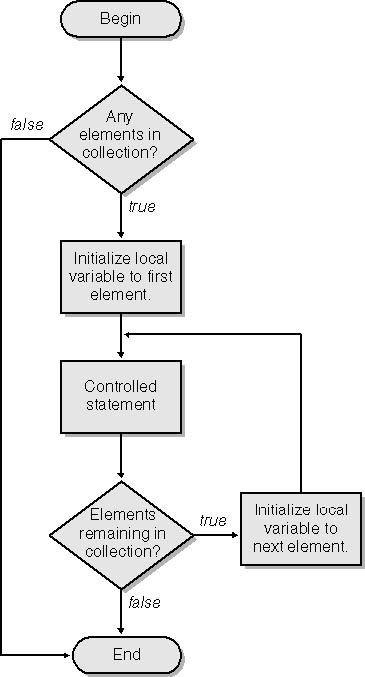
\includegraphics[width=0.5\textwidth]{FqKSJ.jpg}
    \caption{idée de flowchart "for each"}
    \label{flowchart}
\end{figure}
\newpage

\clearpage
\section{Présentation de la version serveur: gestion des utilisateurs et base de données des interactions élèves}

\begin{enumerate}
    \item Une base de données à vocation didactique
    \item Une base de données à vocation pédagogique
    \item Une base de données qui est utilisée: recherche d'optimisations pour améliorer l'expérience utilisateur
\end{enumerate}

vocation didactique : des données exploitables $\Rightarrow$ fiables et assez riches...

vocation pédagogique : gestion des utilisateurs, fiable et éthique, pour être capable de donner rétroaction individuelle en traçant parcours élève...

\subsection{Défi : gérer l'état de l'interface (conditions de concurrence : imprévisibilité)}

\subsubsection{Problèmes identifiés}
\subsubsection{La solution implémentée}

\clearpage
\section{Discussions et conclusions}

\subsection{Critiques Anticipées... et Réponses}
Les objections qui pourraient être faites: expliciter des choix assumés, notes des limitations actuelles dont les solutions ont déjà été pensées et non encore implémentées, des approches alternatives (en cours de recherche ou à l'état complètement hypothétitque)

\subsection{Travaux pour améliorer l'approche actuelle}

\begin{itemize}
    \item Enrichir les types d'exercices et la section "Défis": 
    \begin{enumerate}
        \item Proposer une option "Debug" qui génère des codes invalides, avec des boucles infinies ou syntaxiquement incorrects, appelant les élèves à identifier les erreurs selon leur type.
        \item Des questions qualitatives qui peuvent être ouvertes ou fermées par menu déroulant : Quels sont les types des variables ? (les types étant à récupérer depuis le générateur de code).
        \item Des questions quantitatives \textit{in situ} : Combien de passages dans la boucle ? Combien de passages à tel point du code ?
        \item Des questions mobilisant des concepts théoriques : Telle boucle du code est-elle bornée ? 
    \end{enumerate}

    \item Proposer des QCM sur le code généré, avec erreurs attendues mélangées avec la bonne réponse et des erreurs totalement \textit{random}.
    
    \item Améliorer les rétroactions pour le bouton "Vérifier":
    \begin{enumerate}
        \item Utiliser la réponse élève pour l'analyser au regard des erreurs attendues pour donner des indices (cf. litérature didactique)
        \item Ajouter des \textit{tooltips} (visibles en survolant l'espace de réponse avec le pointeur souris) pour donner des indications de réponses ou des bonnes questions à se poser, pour baliser le travail des élèves
    \end{enumerate}
    
    \item Améliorer l'interface pour renforcer l'engagement :
    \begin{enumerate}
        \item Rendre le \textit{flowchart} cliquable pour un meilleur rendu smartphone
        \item Améliorer la \textit{responsiveness}, notamment les espaces horisontaux pris par les cartes en haut de page
        \item Utiliser des "combines addictives" pour faire revenir les \textit{users}
    \end{enumerate}

    \item Préparer la base de données pour le suivi \underline{de l'évolution des élèves} \textbf{et pour} le suivi \underline{des codes générés} \textbf{et pour} le suivi \underline{des interactions "Défis"}

    \item Améliorer le rendu \textit{flowchart}:
    \begin{itemize}
    
    \item Éléments syntaxiques Python à implémenter : 
    \begin{enumerate}
        \item le \textit{break} à connecter au nœud terminal de sa boucle
        \item les \code{try: except: else: finally:}, les \code{Raise}, les \code{Assert}, ...
        \item Un traitement des annotations de type ?
        \item un traitement de la récursion ?
    \end{enumerate}
    
    \item numéroter les nœuds graphique selon \texttt{lineno} pour visualiser correspondance syntaxe $\Leftrightarrow$ sémantique
    
    \item colorer les flèches "True / False" resp. Bleu/Rouge
    
    \item clarifier (coloriser?) les rendus grpahiques des différents types d'appels: internal\_call, appels de type I/O, ...

    \item animer les éléments graphique ?
    \end{itemize}
    
\end{itemize}


\subsection{Travaux pour une nouvelle approche de génération de code}

------------------------------------------------------
\section{Stack technologique: choix \& hypothèses}

\subsection{UI}

\begin{enumerate}
    \item Chargement des dépendances (parmi tous les possbles pour exécuter du Python dans le navigateur, préférence = $Pyodide$, et en plus $Skulpt$ si besoin) $+$ la jungle des frameworks pour affichage "joli": gros travail de debugging à prévoir même avec $LABjs$
    
    \item Des \texttt{checkbox} pour choisir les \textit{templates}, avec une logique d'exclusion de choix mutuellement exclusifs à définir et à implémenter (si et seulement si la boucle $for$ est choisie il existe la possibilité d'imbriquer des boucles, autre exemple selon le niveau de difficulté choisie on peut griser ou rendre visible certains choix, etc.)
    
    \item Les deux vues  \texttt{script} dans un éditeur de code, et \texttt{flowchart} si implémentées: onglets ou $toggle$ entre les \texttt{<div>}.
    
    \item Pour la présentation du feedback élève à renvoyer après enregistrement des réponses élèves: coloration des cellules $+$ modales pour retours ad hoc, notamment selon comparaison avec erreurs attendues
    
    \item Une piste: les \texttt{tooltips}, pour ajouter des \texttt{mouseover} sur les tokens du code, si possibilité d'y avoir accès... Autre piste: à la création de l'arbre syntaxique, possibilité de récupérer les annotations des noeuds par les parseurs Python
\end{enumerate}

\subsection{Pistes et Hypothèses spécifiques flowchart... desquelles dépendra la logique de génération du code!}

Des solutions très difficiles à créer from scratch, ou des solutions difficiles qui alourdissent la stack.

\begin{enumerate}
    \item Manipuler directement le DOM de l'UI via Pyodide: créer les éléments HTML appropriés et concevoir leur manipulation (= réinventer la roue, puisque des bibliothèques spécialisées ont été créées pour ça)... $\Rightarrow$ idées suivantes:
    \item Bibliothèques JS existantes, exemple $Mermaid.js$: il faut que Python communique le flowchart à Mermaid $\rightarrow$ d'où l'idée du parsing AST
    \item $Graphviz$ et son $DOT language$: à ma connaissance en WebAssembly (accessoirement alourdirait le chargement de la page) donc \textit{à ma connaissance} impossibilité de modifier le DOM directement rendant compliquée (impossible?) l'option du rendu dynamique du flowchart... MAJ 26/03/25 des modules Python existeraient pour faire le travail demandé: cf. \url{https://github.com/pydot/pydot}
\end{enumerate}

\subsection{Génération du code - des idées de pistes avec une supposition à questionner sur le besoin de travailler l'AST correspondant}

Différentes approches à envisager, pas forcément mutuellement exclusives.

\begin{description}
    \item[Approche texte + \texttt{ast}:] Le générateur de code créerait le script à afficher (texte) par application de \textit{templates} préddéfinis en les remplissant au fur et à mesure avec les variables et structures sélectionnées aléatoirement (exemple: "\texttt{if <condition> : <indent> <bloc>}). Approche la plus accessible et la plus facile à controler pédagogiquement, et la plus intuitive pour la production du script car on travaille du texte (ce que l'on veut en sortie) mais il manque le lien logique pour nous rapprocher du flowchart: besoin d'analyser la syntaxe du code généré pour en extraire la structure du code! C'est ce que promettent des fonctions comme \texttt{ast.parse()} pour retourner la racine de l'arbre syntaxique, et la classe \texttt{ast.NodeVisitor} pour parcourir les noeuds intéressants à traduire en noeuds flowchart (pour en garder que les éléments ciblés par nos objetifs pédagogiques). Pyodide est sensé nous donner la possibilité de créer et manipuler les éléments HTML correspondants, à styliser avec une classe CSS correspondante (à définir... plus facile à dire qu'à faire: il faudra supporter l'ancienneté des navigateurs installés dans les écoles et les terminaux des élèves iOS v18 et plus...).
     
     \item[Approche naïve:] S'inspirer de \cite{fuzzingbook} qui semble choisir des productions grammaticales correctes, mais à la signification aléatoire. 

     \item [Approche AST radicale:] Générer un AST pour le traduire en Python et le traduire en flowchart = utiliser l'AST comme une sorte de DSL en faisant une application intensive du module \texttt{ast}. Approche inspirée de ce que j'ai compris de \url{https://github.com/radomirbosak/random-ast}. Utiliser l'arbre assurerait une cohérence syntaxique par rapport au langage (et permettrait des erreurs $Index Error$ ou $Division by zero$ et d'autres plus difficiles à contrôler). Le module \texttt{astor} semble faire le job de traduire l'arbre en code (cf. \url{https://pypi.org/project/astor/}). Le problème principal est la difficulté de créer le générateur d'arbre AST ! Sans parler de la difficulté de le maintenir pérenne selon les mises à jour Python !
     
    \item[Approche via DSL radicale:] D'après \url{https://en.wikipedia.org/wiki/Domain-specific_language} il s'agit d'une solution standard dans l'industrie logicielle de concevoir un DSL adapté à un problème spécifique afin de faciliter la génération de solutions... mais qui semble totalement hors de portée, dépassant le cadre de ce projet, à moins d'en trouver un clé en main !
    
\end{description}

\newpage



\subsection{Fonctionnalités TODO}

\begin{itemize}
    \item Y a-t-il différents types d'utilisateurs ? $\longrightarrow$ oui et non: 
    \begin{enumerate}
        \item oui: enseignants et élèves n'auront pas le même usage
        \item non: enseignants et élèves partagent la même interface et les mêmes fonctionnalités
    \end{enumerate}
    \item Formuler les fonctionnalités sous la forme : 
    \begin{enumerate}
        \item Enseignants \textbf{ET} élèves peuvent :
        \begin{itemize}
            \item utiliser l'outil sur les machines fournies à l'école pour générer des \textit{code snippets}, et regénérer à l'infini
            \item sélectionner les éléments du langage à mobiliser pour chaque code qui sera généré
            \item afficher le code sous forme Python et/ou \textit{flowchart}, au choix
            \item afficher les valeurs des variables en fin de script
            \item sauvegarder localement (pour plus tard) codes et flowcharts jugés intéressants
            \item modifier le code Python généré automatiquement pour l'afficher en flowchart, pour l'évaluer, pour l'exporter, et revenir au code généré initialement
        \end{itemize}
        \item "En tant qu'enseignant, je peux ..." en plus des éléments ci-dessus:
        \begin{itemize}
            \item utiliser les codes générés pour préparer des questions pour animer un cours dialogué, pour interroger les élèves en classe, ou pour impressions (asynchrone)
            \item types d'exercices envisagés: lecture de code Python ; lecture de flowcharts ; traduction d'un langage à l'autre ; code à modifier pour obtenir un certain résultat attendu (prédéfini par l'enseignant)
            \item laisser les élèves être autonomes dans leur progression, rendre les élèves conscients que c'est l'ordinateur qui "donne la réponse"
            \item rendre les élèves conscients des contenus (les éléments à cocher/décocher) et du caractère \textit{presque scientifique} de la démarche
        \end{itemize}
        \item "En tant qu'élève, je peux ..." en plus des éléments ci-dessus:
        \begin{itemize}
            \item m'exercer à la lecture de code Python et à la lecture de flowchart, par l'évaluation de variables en fin de script, de façon autonome avec une rétroaction (juste ou faux)
            \item investiguer des modification du code Python et voir leur effet sur le flowchart et sur les valeurs des variables en sortie du script
            \item bénéficier d'une rétroaction plus riche en cas d'erreur (validation des types? erreurs attendues comme l'indexation pré-évaluées?)
            \item utiliser la plateforme à l'école, sur smartphone, sur tablette et autres écrans personnels (\textit{fully responsive design})
        \end{itemize}
    \end{enumerate}
\end{itemize}

\newpage

\section{Comparaison: \texorpdfstring{MyCFG $\neq$ PyCFG}{MyCFG != PyCFG}}

Nommage des fichiers .py à l'heure d'écriture : \newline
\begin{itemize}
    \item fichier PyCFG.py = Andreas Zeller ("fuzzingbook") puis Rahul Gopinath (etc.) contenant les classes CFGNode et PyCFG, que j'ai à peine modifié pour le rendre fonctionnel dans mon environnement (imports modules + compatibilité 'script' et pas 'Notebook').
Je cite FuzzingBook:
\begin{quote}
    CFGNode representing each node in the control flow graph (...) Next, the PyCFG class which is responsible for parsing, and holding the graph.
\end{quote}
    \item Mon fichier: maintenant nommé MyCFG.py :) contenant une seule classe (hypertrophiée) ControlFlowGraph.
\end{itemize}

%\renewcommand{\arraystretch}{1.2} % un peu d'espace vertical
\noindent\textbf{Ci-dessous : tableau comparatif}
%\vspace{0.5cm}

\begin{longtable}{|p{3cm}|p{7cm}|p{6cm}|}
  \caption{Comparaison des logiques de construction de graphe de flot de contrôle}
  \label{tab:comparatif}
  \\ \hline
  \textbf{Aspect} & \textbf{MyCFG} & \textbf{PyCFG} \\
  \hline
  \endfirsthead

  \multicolumn{3}{l}{\small\slshape Suite du tableau \ref{tab:comparatif}}\\
  \hline
  \textbf{Aspect} & \textbf{MyCFG} & \textbf{PyCFG} \\
  \hline
  \endhead

  \hline
  \multicolumn{3}{r}{\small\slshape Table suite en page suivante} \\
  \endfoot

  \hline
  \endlastfoot

  % ============ contenu du tableau ============
\textbf{Philosophie générale} & 
Analyse directe de l'AST Python, au plus proche de la syntaxe du code source, approche qui se veut pédagogique car tolérante (accepte des chaînes non valides avec \texttt{return} hors d'une définition) & 
Analyse plus sémantique, mais \texttt{lineno} visualisé à chaque nœud; reconstruit le flot d'exécution réel, "désucre" les structures (ex: for $\rightarrow$ while + next), pédagogique mais plus exigente au sens où elle révèle des "détails", plus bas niveau ! \\
\hline
\textbf{Entrée acceptée} & 
Une chaîne de caractères représentant un code Python \textbf{syntaxiquement valide} (y compris invalide, tant que l'AST peut être construit) & 
Uniquement du code Python valide (car lorsqu’il rencontre un return, il cherche à rattacher ce nœud à la fonction englobante en remontant la pile (liste Python) des parents, donc si le return n’est pas dans une fonction (cf. mes \texttt{exemples.py} comme dans NestedIf), la pile des parents finit par être vide, ce qui provoque un \texttt{IndexError} et pas un \texttt{SyntaxError: 'return' outside function}  \\
\hline
\textbf{Construction du graphe} & 
Plusieurs visites de l'AST, chaque structure (If, For, While, etc.) a sa méthode dédiée (\texttt{visit\_If}, \texttt{visit\_For}, ...) & 
Similaire (cf. classe \texttt{PyCFG}) avec  méthodes nommées \texttt{on\_NodeType} (ex: \texttt{on\_if}, \texttt{on\_for}, ...) pour chaque type de nœud AST \\
\hline
\textbf{Gestion des branches et jonctions} & 
Ajoute explicitement des nœuds de jonction pour les structures de contrôle (type \texttt{Junction} pour chaque If, For et While), gère ce qui est sensé représenter une sortie terminale (\texttt{Return}); A MODIFIER: applique la même gestion à \texttt{Break} et \texttt{continue} & 
Suit le flot réel, relie les nœuds selon l’exécution, gère les retours et les sorties via la structure du graphe et la pile de parents. Pas de nœud terminal \texttt{End} pour le flowchart, autre que les \texttt{return} de la fonction définie. \\
\hline
\textbf{Gestion des boucles} & 
Représente les boucles telles qu'elles apparaissent dans le code source (ex: \texttt{For i in ...}) & 
Transforme les boucles \texttt{for} en séquence équivalente (syntaxe un peu cryptique: \texttt{iter}, \texttt{next}, \texttt{while}), chaque étape devient un nœud \\
\hline
\textbf{Gestion des appels de fonction (hors définition de fonction)} & 
Si l'appel est interprété comme tel par l'AST alors affiché de façon spécifique (parallélogramme), sinon affectation simple (rectangle), NB: rendu visuel différent selon que l'appel est avant ou après la déf° (cf. exemples \texttt{defif} et \texttt{defif2}). POUR LE MOMENT: pas différencié appels internes/externes, mais parait faisable & 
Appels de fonctions natives sont comme affectations classiques (rectangles simples); appels des fonctions internes: suivis par le flux de la définitino de fonction. NB: \texttt{return} est un ovale "exit", même si suivi par du code. \\
\hline
\textbf{Gestion des définitions de fonctions} & 
Problématique quand le code est uniquement une définition de fonction ! Les nœuds \texttt{Start} et \texttt{End} sont alors artificiels... logique à redéfinir ??  & 
Impeccable. Caveat idem ci-dessus ! \\
\hline
\textbf{Tolérance aux erreurs} & 
Tolère des return en dehors des fonctions & 
Requiert du code Python syntaxiquement valide pour fonctionner (ex: expressions avec variables non intitialisées ne lèvent psa d'exception) \\
\hline
\textbf{Sortie / Visualisation} & 
Génère une chaine en syntaxe Mermaid (un DOT language similaire à Graphviz) mieux adaptée pour un rendu Web il me semble: plus facile à maintenir & 
Génère du DOT-Graphviz: infrastrucutre plus lourde! à décortiquer pour rendre un Mermaid\_{JS} mais visualisation avancée, couleurs et styles selon le flot \\
\hline
\textbf{Gros Pour} & 
plus souple = plus proche de ce qui est fait en classe ; infrastructure légère & 
visualisation plus propre (eg: flux principal vs \texttt{def})  \\
\hline
\textbf{Gros Contre} & 
encore bugs et incertitudes... & 
c'est Digraph qui fait le graph !! \\
\hline

  % ========== fin du contenu ==========
\end{longtable}

\section{Documentation du 28 avril: fichier \texttt{MyCFG} }

\begin{longtable}{| >{\bfseries}l | p{4cm} | p{7cm} |}
\caption{Correspondance des Types de Nœuds Internes, Nœuds AST et Sémantique}\label{tab:node_types}\\
\hline
\textbf{Node Type (Interne)} & \textbf{Nœud(s) AST Correspondant(s)} & \textbf{Sémantique (Langage Naturel)} \\
\hline
\endfirsthead
\hline
\endfoot
\hline
\multicolumn{3}{r}{\small\slshape Table suite en page suivante} \\
\hline
\endlastfoot
% --- Types Implémentés --- & & \\ \hline
StartEnd & \texttt{ast.Module} (implicite), \texttt{ast.FunctionDef} (implicite) & Représente le point d'entrée ('Start') ou de sortie ('End') global du script/module ou d'une fonction spécifique. \\ \hline
Decision & \texttt{ast.If}, \texttt{ast.While}, \texttt{ast.For} & Nœud où le flux de contrôle se divise en fonction d'une condition (If, While) ou de l'état d'une itération (For, While). Représenté typiquement par un losange. \\ \hline
Process & \texttt{ast.Assign}, \texttt{ast.Expr}, \texttt{ast.Call}, et autre non implémentés via \texttt{generic\_visit}: \texttt{ast.Pass}, \texttt{ast.Delete}, \texttt{ast.Import}, \texttt{ast.ImportFrom} & Représente une étape d'exécution séquentielle : une affectation, l'évaluation d'une expression, un appel de fonction, une instruction vide (\texttt{pass}), une suppression, un import, etc. Représenté typiquement par un rectangle. \\ \hline
Junction & N/A (Nœud structurel ajouté) & Point de convergence où plusieurs chemins d'exécution se rejoignent (souvent après un 'If/Else') ou point de sortie défini d'une boucle. Représenté typiquement par un petit cercle ou un point. \\ \hline
Return & \texttt{ast.Return} & Indique la fin de l'exécution d'une fonction et potentiellement le retour d'une valeur. Termine le chemin d'exécution dans cette fonction. Représenté par une forme spécifique (parallélogramme incliné, etc.). \\ \hline
Jump & \texttt{ast.Break}, \texttt{ast.Continue} & Représente un saut inconditionnel dans le flux de contrôle vers un autre point défini (sortie de boucle pour 'Break', début de l'itération suivante pour 'Continue'). Termine le chemin séquentiel *local*. Représenté par un cercle ou une note. \\ \hline
Subroutine & \texttt{ast.FunctionDef} & Représente la *définition* d'une fonction (sa signature). Peut être lié au flux principal pour montrer où elle est définie. Représenté par un parallélogramme ou un rectangle avec des barres. \\ \hline
\\ \hline
% --- Types à Implémenter (en vrac, pas exhaustif) --- & & \\ \hline

ExceptionHandler & \texttt{ast.ExceptHandler} (dans \texttt{ast.Try}) & Bloc de code exécuté lorsqu'une exception spécifique est attrapée dans un bloc 'Try'. \\ \hline
TryBlock & \texttt{ast.Try} (partie \texttt{body}) & Le bloc de code principal surveillé pour les exceptions. \\ \hline
FinallyBlock & \texttt{ast.Try} (partie \texttt{finalbody}) & Bloc de code qui est *toujours* exécuté après un bloc 'Try', qu'une exception ait eu lieu ou non. Modifie le flux de sortie. \\ \hline
ElseBlock (Try/Loop) & \texttt{ast.Try} (partie \texttt{orelse}), \texttt{ast.For}/\texttt{ast.While} (partie \texttt{orelse}) & Bloc exécuté si *aucune* exception n'est levée dans le 'Try' correspondant, ou si une boucle se termine *normalement* (sans 'Break'). \\ \hline
Raise & \texttt{ast.Raise} & Provoque un saut inconditionnel hors du flux normal vers un gestionnaire d'exception ou termine le programme si non attrapé. Termine le chemin séquentiel local. \\ \hline
ContextManager (With) & \texttt{ast.With}, \texttt{ast.AsyncWith} & Gère l'entrée et la sortie d'un contexte (ex: ouverture/fermeture de fichier). Représente un bloc avec potentiellement du code setup/teardown implicite. \\ \hline
Assertion & \texttt{ast.Assert} & Vérifie une condition et lève une \texttt{AssertionError} si elle est fausse. Peut être vu comme une Décision menant potentiellement à un 'Raise'. \\ \hline
ClassDefinition & \texttt{ast.ClassDef} & Similaire à 'Subroutine', représente la définition d'une classe. \\ \hline
Yield & \texttt{ast.Yield}, \texttt{ast.YieldFrom} & Spécifique aux générateurs, met en pause l'exécution et retourne une valeur, permettant la reprise ultérieure. Modifie profondément le flux. \\ \hline
AsyncAwait & \texttt{ast.AsyncFunctionDef}, \texttt{ast.Await}, \texttt{ast.AsyncFor}, \texttt{ast.AsyncWith} & Constructs pour la programmation asynchrone, impliquant des points de suspension et une boucle d'événements. (Probablement hors de portée initiale). \\ \hline

\end{longtable}
\newpage

\section{Documentation des modifs UI du 24/06/25}
Défis rencontrés : \begin{itemize}
    \item Garantir que l'état visuel de l'interface reflète toujours de manière fiable la synchronisation entre le code dans l'éditeur et le diagramme affiché, à la condition que le flowchart soit effectivement modifié (pas pour les changement cosmétiques, non sémantiques); 
    \item L'état "périmé" (outdated) n'a de sens que s'il y a un diagramme de référence à comparer. Si nous rechargeons le code, nous invalidons de fait le diagramme précédent.
    \item Arriver à un code plus cohérent qui élimine la "condition de concurrence" (race condition) qui se produit lorsque des estionnaires d'événements accèdent à - et manipulent - l'état visuel des bordures, et que le résultat final dépend de l'ordre, imprévisible, dans lequel ils s'exécutent. 
\end{itemize}

\textbf{Petit scénario explicatif de la concurrence par la métaphore de la "course" (race condition):}
1. Le problème avec le bouton 'reload':
Le "coureur" n°1 démarre : Le gestionnaire d'événement du bouton reload-code-btn est appelé.
Le "coureur" n°1 agit : Il exécute la ligne codeEditorInstance.setValue(lastLoadedCode).
Le "coureur" n°2 est déclenché : L'action setValue déclenche immédiatement l'événement change de l'éditeur de code. Le gestionnaire codeEditorInstance.on('change', ...) se met en route.
Le "coureur" n°2 agit :
Il récupère le nouveau code.
Il calcule son AST.
Il le compare à lastDiagramAstDump, qui contient toujours l'AST de l'ancien code (celui d'avant le rechargement).
La comparaison échoue ! Les AST sont différents.
Le "coureur" n°2 conclut donc que le diagramme est périmé et appelle setDiagramAndChallengeCardState("outdated"). Les bordures deviennent rouges.
Le "coureur" n°1 termine sa course : Après que le "coureur" n°2 a fini, le gestionnaire du bouton "Reload" reprend et exécute sa dernière ligne : setDiagramAndChallengeCardState("default").
Le Résultat ? Le plus souvent, le "coureur" n°2 (le change handler) était plus rapide ou son effet visuel s'appliquait en dernier, laissant les bordures rouges. Le résultat était imprévisible et dépendait du timing du navigateur. C'était une course, et le mauvais coureur gagnait.
2. LA solution: pas faire courir les processus plus vite, mais changer les règles de la course pour qu'elle devienne une coopération orchestrée.
1) Invalider l'État de Référence en Premier
Dans le nouveau code du reload-code-btn, la toute première chose que nous faisons est :
lastDiagramAstDump = "";
C'est l'équivalent de dire : "Attention, le diagramme qui était affiché n'a plus aucune valeur. Il n'y a plus de référence valide."
2) Rendre le \texttt{change} Handler plus "Intelligent"
Le gestionnaire codeEditorInstance.on('change', ...) a maintenant une nouvelle instruction au tout début de son code :
\begin{minted}{Javascript}
if (!lastDiagramAstDump) {
    setDiagramAndChallengeCardState("default");
    return; // Arrête-toi ici !
}
\end{minted}
i.e. "Avant de faire quoi que ce soit, vérifie s'il existe un diagramme de référence valide. Si lastDiagramAstDump est vide, le diagramme est invalidé. Ton seul travail est de t'assurer que les bordures sont bleues (default) et de t'arrêter immédiatement. Ne continue pas la comparaison des AST."

Continuons la métaphore avec des "coopérateurs" et non des coureurs concurrents:
Le "coopérateur" n°1 démarre : Le gestionnaire du reload-code-btn est appelé.
Le "coopérateur" n°1 prépare le terrain : Il exécute immédiatement lastDiagramAstDump = "". L'état de référence est maintenant invalidé. C'est le passage de témoin.
Le "coopérateur" n°1 continue : Il appelle codeEditorInstance.setValue(lastLoadedCode).
Le "coopérateur" n°2 est déclenché : L'événement change est émis.
Le "coopérateur" n°2 lit les instructions :
Il entre dans sa logique et sa première question est : if (!lastDiagramAstDump).
La réponse est VRAI ! Le "coopérateur" n°1 a bien invalidé la variable.
Il exécute donc setDiagramAndChallengeCardState("default") (les bordures deviennent bleues) et s'arrête net grâce au return.
Fin de l'opération : Le gestionnaire change a terminé son travail correctement. Le gestionnaire reload termine aussi. Le résultat final est stable, prévisible et correct : les bordures sont bleues.

Bref, la liste des modis effectuées:
\begin{enumerate}
    \item setDiagramAndChallengeCardState(state) :
    \begin{itemize}
        \item Légèrement modifiée pour être plus robuste : elle retire d'abord toutes les classes de bordure potentielles (border-danger, border-info, etc.) ainsi que la classe border de base, avant de réappliquer les bonnes. Cela évite d'avoir plusieurs classes de bordure en même temps.
        \item Utilise \texttt{?.closest('.card')} pour éviter une erreur si l'élément n'est pas trouvé dans le DOM.
    \end{itemize}
    
    \item lastDiagramAstDump (Variable Globale) :
    \begin{itemize}
        \item Cette variable est maintenant la seule source de vérité pour l'état du diagramme affiché.
        \item Elle est initialisée à "" (chaîne vide).
        \item Elle n'est mise à jour que lors d'un clic réussi sur le bouton "Lancer ...".
        \item Elle est invalidée (remise à "") chaque fois qu'un nouveau code est chargé, généré ou rechargé, car le diagramme ne correspond plus.
    \end{itemize}

    \item Listener du bouton "Lancer..." (run-code-btn) :
    \begin{itemize}
        \item C'est ici que lastDiagramAstDump est mis à jour avec le ast.dump du code qui vient d'être exécuté pour générer le diagramme.
        \item Après cette mise à jour, il appelle \texttt{setDiagramAndChallengeCardState("default")} pour mettre les bordures en bleu, car le code et le diagramme sont maintenant synchronisés.
    \end{itemize}

    \item Listener du bouton "Reload" (reload-code-btn) :
    \begin{itemize}
        \item C'est le cœur de la correction. La logique est maintenant :
        \begin{enumerate}
            \item Invalider l'état du diagramme en premier : lastDiagramAstDump est remis à "" et le contenu du div $\#flowchart$ est effacé.
            \item Ensuite, mettre à jour le code dans l'éditeur : codeEditorInstance.setValue(lastLoadedCode).
        \end{enumerate}
        \item \textbf{Pourquoi cet ordre est-il crucial ?} Lorsque \texttt{setValue} est appelé, l'événement \texttt{change} de l'éditeur se déclenche immédiatement. Ce listener (décrit ci-dessous) verra que \texttt{lastDiagramAstDump} est vide et mettra l'état visuel à "default", ce qui est exactement le comportement souhaité. La course est ainsi gagnée en préparant l'état avant de déclencher l'événement !
    \end{itemize}

    \item Listener \texttt{change} de \texttt{codeEditorInstance} :
Sa logique a été affinée :
    \begin{itemize}
        \item a. Il vérifie d'abord si lastDiagramAstDump est vide/invalide. Si c'est le cas, cela signifie qu'il n'y a pas de diagramme de référence. L'état est donc forcément "default" (on ne peut pas être "périmé" par rapport à rien). Il met les bordures en bleu et s'arrête.
        \item b. Ce n'est que si lastDiagramAstDump a une valeur qu'il procède à la comparaison des AST et met l'état à "outdated" si nécessaire.
    \end{itemize}
    \end{enumerate}
\newpage

\section{Documentation des modifs \texttt{code-generator.js} du 30/06/25}

\subsection{Objectifs du générateur}

\begin{itemize}
    \item Générer du code Python syntaxiquement correct et exécutable
    \item Adapter la complexité selon le niveau souhaité
    \item Permettre la sélection précise d'éléments syntaxiques
    \item Produire du code pédagogiquement pertinent
    \item Offrir une variété suffisante pour des exercices diversifiés
\end{itemize}


\subsection{Flux d'exécution du processus de génération actuel}
TODO: Debug indentation dans ForRange \newline
Le processus de génération suit ces étapes principales:

\begin{enumerate}
    \item L'utilisateur configure les options dans l'interface (types de variables, structures de contrôle, etc.)
    \item Le bouton "Générer un Code Aléatoire" déclenche la collecte des options
    \item La fonction \texttt{generateRandomPythonCode(options)} est appelée par \texttt{main.js}
    \item Cette fonction est définie dans \texttt{code-generator.js}
    \item Le générateur crée le code en plusieurs phases:
    \begin{enumerate}
        \item Initialisation des constantes et variables
        \item Calcul des lignes requises pour les structures demandées
        \item Préparation des variables nécessaires
        \item Génération des structures de contrôle
        \item Complétion pour atteindre le nombre de lignes cible
    \end{enumerate}
    \item Le code généré est retourné à l'interface
    \item L'utilisateur peut alors simuler l'exécution du code, visualiser le diagramme et répondre aux défis.
\end{enumerate}

\subsection{Principales fonctions de génération }

Implémentées actuellement:
\begin{longtable}{p{5cm}p{10cm}}
\toprule
\textbf{Fonction} & \textbf{Description} \\
\midrule
\texttt{generateRandomPythonCode} & Fonction principale de génération qui orchestre tout le processus \\
\texttt{calculateRequiredLines} & Calcule le nombre minimum de lignes nécessaires \\
\texttt{ensureVariablesForOptions} & Crée les variables demandées par l'utilisateur \\
\texttt{ensureRequiredVariables} & Garantit que les variables nécessaires aux structures sont présentes \\
\texttt{generateControlStructures} & Génère les structures de contrôle (if, boucles, fonctions) \\
\texttt{generateIfStatement} & Génère une structure conditionnelle if/elif/else \\
\texttt{generateForRangeLoop} & Génère une boucle for avec range() \\
\texttt{generateForListLoop} & Génère une boucle for parcourant une liste \\
\texttt{generateForStrLoop} & Génère une boucle for parcourant une chaîne \\
\texttt{generateWhileLoop} & Génère une boucle while \\
\texttt{generateFunction} & Génère une définition de fonction \\
\texttt{addFiller} & Ajoute des opérations simples pour atteindre le nombre de lignes cible \\
\bottomrule
\end{longtable}

Actuellement abandonnées:
\begin{longtable}{p{5cm}p{10cm}}
\toprule
\textbf{Fonction} & \textbf{Description} \\
\midrule
\texttt{generateSimpleOperation} & Fonction qui écrit un minimum de code \\
\texttt{planVariable} & Fonction de gestion de la présence des variables nécessaires \\
\texttt{ensureVariableForStructure} & Fonction qui crée les variables demandées par les structures sélectionnées \\
\texttt{finalVariableCheck} & ... \\
\texttt{availableForVariables} & variable de stockage  \\
\bottomrule
\end{longtable}

\subsection{Stratégie actuelle de gestion des variables}
La gestion des variables est encore problématique, c'est l'un des aspects les plus complexes du générateur. Elle repose sur plusieurs mécanismes:

\begin{itemize}
    \item Les variables sont stockées dans \texttt{declaredVarsByType}, un objet qui les classe par type
    \item Un ensemble \texttt{allDeclaredVarNames} permet de vérifier l'unicité des noms
    \item Les variables planifiées mais non encore déclarées sont stockées dans \texttt{plannedVarsByType}
    \item Des fonctions utilitaires générent des noms uniques et des valeurs appropriées
\end{itemize}

Résultat: plusieurs problèmes !
\begin{enumerate}
    \item \textbf{Problème d'indentation déjà mentionné}: La fonction \texttt{ensureVariableExists()} ne respecte pas l'indentation courante lors de la création de variables dans des structures de contrôle.
    
    \item \textbf{Fonctions redondantes}: Plusieurs fonctions coexistent avec des rôles similaires:
    \begin{itemize}
        \item \texttt{finalVariableCheck()} n'est finalement jamais appelée dans le flux d'exécution actuel
        \item \texttt{ensureVariableForStructure()} redondante avec \texttt{ensureVariableExists()}
        \item \texttt{generateSimpleOperation()} similaire à \texttt{generateAppropriateStatement()}
        \item \texttt{generateVariables()} et \texttt{ensureVariablesForOptions()} ont des rôles qui se chevauchent
    \end{itemize}
    
    \item \textbf{Variables inutilisées}: \texttt{availableForVariables} est calculée mais jamais utilisée
    
    \item \textbf{Distinction confuse}: La distinction entre variables "déclarées" et "planifiées" qui était prévue n'est pas toujours clairement respectée dans le code
\end{enumerate}

\subsection{Solutions proposées}

Pour résoudre ces problèmes, les modifications suivantes sont recommandées:

\begin{enumerate}
    \item \textbf{Correction de \texttt{ensureVariableExists()}}: Modifier cette fonction pour qu'elle tienne compte de l'indentation courante et ajoute les variables avant les structures de contrôle:
    
    \begin{minted}{javascript}
function ensureVariableExists(type, preferPlanned = false) {
    // Si on est dans une structure (indentLevel > 0)
    if (indentLevel > 0) {
        // Trouver d'abord une variable existante
        if (declaredVarsByType[type].length > 0) {
            return getRandomItem(declaredVarsByType[type]);
        }
        
        // Sinon, créer une variable AVANT la structure
        const name = generateUniqueVarName(type);
        const currentPosition = codeLines.length;
        
        // Trouver l'endroit où insérer la déclaration
        let insertPosition = currentPosition - 1;
        while (insertPosition >= 0 && 
               codeLines[insertPosition].startsWith("    ")) {
            insertPosition--;
        }
        
        // Insérer la déclaration à cet endroit
        codeLines.splice(insertPosition + 1, 0, 
            `${name} = ${LITERALS_BY_TYPE[type](difficulty)}`);
        declaredVarsByType[type].push(name);
        allDeclaredVarNames.add(name);
        linesGenerated++;
        
        return name;
    }
    
    // Comportement normal hors structures
    // ...
}
    \end{minted}
    
    \item \textbf{Simplification des fonctions de gestion des variables}:
    \begin{itemize}
        \item Supprimer \texttt{finalVariableCheck()} et intégrer sa logique dans \texttt{ensureRequiredVariables()}
        \item Remplacer \texttt{ensureVariableForStructure()} par des appels à \texttt{ensureVariableExists()}
        \item Unifier \texttt{generateSimpleOperation()} et \texttt{generateAppropriateStatement()}
        \item Clarifier les rôles de \texttt{generateVariables()} et \texttt{ensureVariablesForOptions()}
    \end{itemize}
    
    \item \textbf{Nettoyage des variables inutilisées}: Supprimer \texttt{availableForVariables} ou l'utiliser effectivement dans le code
    
    \item \textbf{Clarification de la distinction entre variables déclarées et planifiées}:
    \begin{itemize}
        \item Documenter clairement le cycle de vie des variables
        \item Utiliser systématiquement \texttt{declareVariable()} pour passer une variable de "planifiée" à "déclarée"
        \item Vérifier que toutes les variables planifiées sont bien déclarées avant la fin de la génération
    \end{itemize}
\end{enumerate}

\section{Structures de contrôle}

\subsection{Logique de génération des structures}

Les structures de contrôle sont générées selon un processus en deux phases:

\begin{enumerate}
    \item \textbf{Préparation}:
    \begin{itemize}
        \item Construction d'une liste des structures à générer selon les options
        \item Mélange aléatoire de cette liste pour varier l'ordre d'apparition
        \item Vérification et création des variables nécessaires
    \end{itemize}
    
    \item \textbf{Génération}:
    \begin{itemize}
        \item Parcours de la liste des structures
        \item Appel de la fonction appropriée pour chaque structure
        \item Gestion de l'indentation et du comptage des lignes
    \end{itemize}
\end{enumerate}

\subsection{Itérateurs et variables locales}

Un soin particulier est apporté aux variables d'itération:

\begin{itemize}
    \item Les noms d'itérateurs sont générés via \texttt{generateUniqueIteratorName()}
    \item Un compteur global \texttt{iteratorCounter} garantit des noms distincts
    \item Les itérateurs sont traités différemment des variables ordinaires
\end{itemize}

\subsection{Cas particuliers}

\begin{itemize}
    \item \textbf{Boucles for-in-list et for-in-str}: Si l'utilisateur n'a pas spécifié de variables list/str, un littéral est utilisé directement dans la boucle
    \item \textbf{Boucles while}: Une condition décrémentale est générée pour éviter les boucles infinies
    \item \textbf{Conditions if-elif-else}: La parenté entre options est gérée (if-elif implique if, if-elif-else implique if-elif)
\end{itemize}





\begin{thebibliography}{99}

\bibitem{pyodide} Pyodide Development Team. (2023). \textit{Pyodide Documentation}. Récupéré de \url{https://pyodide.org} (consulté en 2024).

\bibitem{codemirror6} Haverbeke, M. (2021). \textit{CodeMirror 6 Documentation}. Récupéré de \url{https://codemirror.net/6/} (consulté en 2024).

\bibitem{ace} Ace Editor. (n.d.). \textit{Ace - The High Performance Code Editor for the Web}. Récupéré de \url{https://ace.c9.io} (consulté en 2024).

\bibitem{python-ast} Python Software Foundation. (2023). \textit{Python Documentation: ast --- Abstract Syntax Trees}. Extrait de \url{https://docs.python.org/3/library/ast.html} (consulté en 2024).

\bibitem{python-dis} Python Software Foundation. (2023). \textit{Python Documentation: dis --- Disassembler for Python bytecode}. Extrait de \url{https://docs.python.org/3/library/dis.html} (consulté en 2024).

\bibitem{kluyver2012} Kluyver, T. (2012). \textit{Green Tree Snakes: Getting to and from ASTs}. Documentation en ligne, \url{https://greentreesnakes.readthedocs.io} (consulté en 2024).

\bibitem{fuzzingbook} Zeller, A. et al. (2022). \textit{The Fuzzing Book} – Chapitre "Fuzzing with Grammars". En ligne, \url{https://www.fuzzingbook.org} (consulté en 2024).

\bibitem{didask} Didask. (n.d.). \textit{Qu'est-ce qu'un outil auteur ? - Le guide complet}. Recopié de \url{https://www.didask.com (consulté en 2025)}.

\bibitem{wenger} Wenger, E. (1998).\textit{Communities of practice: Learning, meaning, and identity}. Cambridge University Press. \url{https://doi.org/10.1017/CBO9780511803932}

\bibitem{papert1980} Papert, S. (1980). \textit{Mindstorms: Children, Computers, and Powerful Ideas}. Basic Books.

\bibitem{messer2023} Messer, M., Brown, N.C.C., Kölling, M., \& Shi, M. (2023). Automated Grading 
and Feedback Tools for Programming Education: A Systematic Review. \textit{arXiv preprint} 
arXiv:2306.11722.

\bibitem{zimmermann2024} Zimmermann, A. E., King, E. E., \& Bose, D. D. (2024). Effectiveness 
and Utility of Flowcharts on Learning in a Classroom Setting: A Mixed-Methods Study. 
\textit{American Journal of Pharmaceutical Education, 88}(1), 100591.

\bibitem{sovietov} Sovietov, P. (2022). Automatic Generation of Programming Exercises. \textit{Institute of Information Technologies MIREA – Russian technological university Moscow, Russia - sovetov@mirea.ru} 10.48550/arXiv.2205.11304. 

\end{thebibliography}

\end{document}
